\chapter{A review on fractional and graph Fourier transforms}
\label{ch:reviewGSP}

At the heart of the field of spectral analysis lies the concept of \textit{Fourier transforms}, all of which are creatively tailored to map the original signal onto convenient new spaces. This links directly to the argument presented in the Introduction of this thesis: the power and flexibility of signal processing stem from the many ways in which one can explore different signal representations. While the last chapter ended with a brief presentation of the QFT, the next pages will guide the reader through an overview on two sets of transforms which are also relevant to understanding the contributions in the thesis: the fractional Fourier transform (FrFT) and the graph Fourier transform, the latter included in the broader discussion on fundamentals of graph signal processing.

\section{The fractional Fourier transform}

It is quite common in theoretical investigations to expand the definition of some well-established operator and consider the consequences of an intermediate (fractional) application of the underlying operation. Take, for example, the power operation, which makes \textit{sense} only for integer exponents (i.~e., $x^3 \overset{\Delta}{=} x \cdot x \cdot x$), but has great use when considering also real or complex exponents. Or the derivative of a function $f(t)$, which can be defined to possess a fractional-order equivalent by setting $n$ to non-integer values in the time differentiation property of the Fourier transform $\mathcal{F} \left\{ \cdot \right\}$:
\begin{equation}
\label{eq:derivative}
\mathcal{F} \left\{ \left[ \frac{\mathrm{d}^n}{(\mathrm{d}t)^n} f(t) \right] \right\} =
(\qj \omega)^n \mathcal{F} \left\{ f(t) \right\}.
\end{equation}
Mendlovic and Ozaktas made this observation \cite{mendlovic1993fractionalI} and pointed out that this was the spark behind the creation of the FrFT. However theoretical this endeavor might have been, even at its origin in the 1980's paper on the Journal of Applied Mathematics by the physicist Victor Namias \cite{namias1980fractional}, the fractional Fourier transform had already potential applications, originally in quantum mechanics. After 40 years, the FrFT has been applied to time-frequency analysis, compression, digital watermarking, filtering, encryption, let alone its utility in Optics \cite{bultheel2002shattered,figueiredo2018}.

The fractional Fourier transform is a generalization of the usual continuous-time Fourier transform and can be interpreted as a rotation of the signal (operand) in the time-frequency plane \cite{almeida1994fractional}. To understand why, let us consider its definition. The usual (unitary) Fourier transform, with operator represented by $\mathcal{F}$ as in (\ref{eq:derivative}), has analysis and synthesis equations given by
\begin{equation}
\mathcal{F}\left\{ f(t) \right\} = F(\qi \omega) = \frac{1}{\sqrt{2 \pi}} \int_{-\infty}^{\infty} f(t) \exp(-\qi \omega t) \mathrm{d}t,
\end{equation}
\begin{equation}
\mathcal{F}^{-1}\left\{ F(\qi \omega) \right\} = f(t) = \frac{1}{\sqrt{2 \pi}} \int_{-\infty}^{\infty} F(\qi \omega) \exp(\qi \omega t) \mathrm{d}\omega.
\end{equation}

The eigenfunctions of the $\mathcal{F}$ operator are the family of functions $\exp (\frac{-x^2}{2}) H_n(x)$ (on the variable $x$), where $H_n(x)$ are the Hermite polynomials of order $n$ \cite{namias1980fractional}. The associated eigenvalues have the form $\exp(- \qj n \frac{\pi}{2})$; therefore, if we add the notation $\mathcal{F}_{\frac{\pi}{2}} \overset{\Delta}{=} \mathcal{F}$,
\begin{equation}
\label{eq:eighermite}
\mathcal{F}_{\frac{\pi}{2}} \left\{ \exp \left(\frac{-x^2}{2}\right) H_n(x) \right\} = 
\exp\left(- \qj n \frac{\pi}{2}\right)
\exp \left(\frac{-x^2}{2}\right) H_n(x).
\end{equation}

The FrFT is then \textit{defined} as the operator $\mathcal{F}_\alpha$ satisfying the eigenvalue equation
\begin{equation}
\label{eq:frftdef}
\mathcal{F}_{\alpha} \left\{ \exp \left(\frac{-x^2}{2}\right) H_n(x) \right\} = 
\exp\left(- \qj n \alpha\right)
\exp \left(\frac{-x^2}{2}\right) H_n(x),
\end{equation}
from which follows that $\alpha = 0$ yields the identity operator and $\alpha = \frac{\pi}{2}$ makes the FrFT coincide with the usual Fourier transform (by definition). The \textit{order} of the fractional Fourier transform is defined by $m = \frac{2\alpha}{\pi}$.

The integral form of the operator $\mathcal{F}_\alpha$ is
\begin{equation}
\label{eq:integralfrft}
\mathcal{F}_\alpha \left\{ f(t) \right\} = \int_{-\infty}^{\infty} f(t) K_\alpha (t, u) \mathrm{d}t,
\end{equation}
in which the transformation kernel $K_\alpha (t, u)$ is given by
\begin{equation}
K_\alpha (t, u) = 
\begin{cases}
\sqrt{\frac{1 - \qj \cot \alpha}{2\pi}} \exp \left( \qj \frac{t^2 + u^2}{2} \cot \alpha - \qj ut \csc \alpha\right), &
\text{if $\alpha$ is not a multiple of $\pi$,} \\
\delta (t - u), & \text{if $\alpha$ is a multiple of $2\pi$,} \\
\delta (t + u), & \text{if $\alpha + \pi$ is a multiple of $2\pi$.}
\end{cases}
\end{equation}

\begin{figure}
\centering
\caption{Illustration of the FrFT property of rotation in the time-frequency plane.}
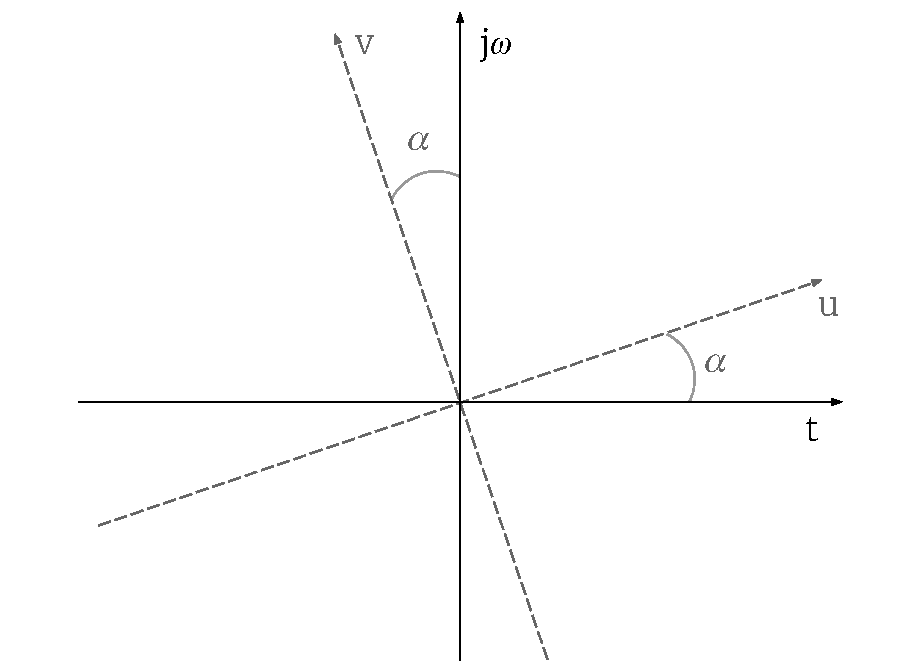
\includegraphics[width=0.65\linewidth]{Figures/FrFT-Rotation-cropped.pdf}
\floatsource[adapted from \cite{almeida1994fractional}]
\label{fig:frft_rotation}
\end{figure}

Two successive applications on the signal $f(t)$ of the FrFT with orders $m_1 = \frac{2\alpha_1}{\pi}$ and $m_2 = \frac{2\alpha_2}{\pi}$ can be written in a single equation as
\begin{align}
\label{eq:frftsucessive}
\mathcal{F}_{\alpha_2} \left\{ \mathcal{F}_{\alpha_1} \left\{ f(t) \right\} \right\} &=
\int_{-\infty}^{\infty} 
\left( \int_{-\infty}^{\infty} f(t) K_{\alpha_1} (t, s) \mathrm{d}t \right)
K_{\alpha_2} (s, u) \mathrm{d}s \\
&= 
\int_{-\infty}^{\infty}
f(t)
\left(
\int_{-\infty}^{\infty}
K_{\alpha_1} (t, s) K_{\alpha_2} (s, u) \mathrm{d}s
\right)
\mathrm{d}t.
\end{align}
After a ``rather long derivation'', according to \cite{almeida1994fractional}, it has been shown that
\begin{equation}
\label{eq:summingangles}
\int_{-\infty}^{\infty}
K_{\alpha_1} (t, s) K_{\alpha_2} (s, u) \mathrm{d}s = 
K_{\alpha_1 + \alpha_2} (t, u),
\end{equation}
and this implies
\begin{align}
\mathcal{F}_{\alpha_2} \left\{ \mathcal{F}_{\alpha_1} \left\{ f(t) \right\} \right\} &=
\int_{-\infty}^{\infty}
f(t)
K_{\alpha_1 + \alpha_2} (t, u)
\mathrm{d}t
= \mathcal{F}_{\alpha_1 + \alpha_2} \left\{ f(t) \right\}.
\end{align}
In other words, the FrFT has the property of additivity of transform orders. Let us see how this fits quite nicely with the known behavior of successive applications of the usual unitary Fourier transform.

It is known that Fourier-transforming twice the same signal yields the operand with reflected time axis,
\begin{equation}
\mathcal{F}^{(2)} \left\{ f(t) \right\} \overset{\Delta}{=}
\mathcal{F} \left\{ \mathcal{F} \left\{ f(t) \right\} \right\}
= f(-t),
\end{equation}
applying the transform once more yields the signal spectrum with reflected frequency axis,
\begin{equation}
\mathcal{F} \left\{ f(-t) \right\} = F(-\qj \omega),
\end{equation}
and further transforming once more gives back the original signal,
\begin{equation}
\mathcal{F} \left\{ F(-\qj \omega) \right\} = f(t).
\end{equation}
It is as if the Fourier transform moved the signal back and forth in 90\textsuperscript{o} degrees rotations in the time-frequency plane. From this point of view, the FrFT may be seen as a general rotation in the time-frequency plane, with $\mathcal{F}_\alpha$ rotating the signal axis by $\alpha$ degrees. A 360\textsuperscript{o} rotation yields
\begin{equation}
\mathcal{F}_{2\pi} \left\{ f(t) \right\} = \mathcal{F}_{
\frac{\pi}{2} + 
\frac{\pi}{2} + 
\frac{\pi}{2} + 
\frac{\pi}{2}
} \left\{ f(t) \right\} =
\mathcal{F}^{(4)} \left\{ f(t) \right\} = f(t),
\end{equation}
which in fact goes ``back'' to the original time axis. See a depiction of the rotation in the time-frequency plane in Fig. \ref{fig:frft_rotation}.

Finally, the additivity of orders guarantees that the inverse of the $\mathcal{F}_\alpha$ exists and equals $\mathcal{F}_{-\alpha}$. Since the fractional transform order is a real-valued parameter, it is quite hard to recover perfectly the original signal from its spectrum if the value of $\alpha$ is unknown. This favors the use of discrete fractional transforms in specific steps of encryption schemes \cite{tao2010image, kang2018reality, kang2018color}.

\section{Fundamentals of graph signal processing}

Multivariate data defined over networks are nowadays ubiquitous, being constantly generated, stored and processed in the most diverse systems in engineering and technology. Measurements in a set of IoT sensors and mobile devices~\cite{alam2015toward,guo2016qos,ma2016non,yu2016novel}, number of citations in a scientific collaboration network or social media relations (\emph{collaboration graph}, or \emph{social graph})~\cite{chung2010graph} and interactions between individuals in a ecosystem (\emph{ecological networks})~\cite{golubski2016} are some examples of situations in which the acquired data are intimately related to the topology of the network over which they are defined.

Such multivariate network-like systems are not only present in various applications, but are also systematically growing in number, as sensors become cheaper and smaller and concepts such as cloud storage/computing and Big Data consolidate, as indicated by the 2011 report from McKinsey Global Institute \cite{mckinsey2011big}. This document also states that the information acquired from the adequate processing of such massive networked data is a fundamental requisite for the companies to thrive from now on.

Still another motivation that feeds the urge to study processing techniques for data defined over network-like domains, for example, is the growth of research on \emph{smart cities}, which takes advantage of the considerable information (that are or are yet to be) generated in cities to provide (or improve the) solutions  for many urban problems \cite{jain2014big}.

All these examples share an important characteristic: the structure over which the data is defined may be modeled by a graph \cite{mei2016signal}, to which vertices are assigned the variables of interest, as depicted in Fig. \ref{fig:duher}. That is the context in which the field of \emph{graph signal processing} (GSP) was developed in the last decade, a theoretical framework aiming to generalize the classical signal processing methods and concepts to scenarios in which the signal is no more defined over a regular domain, but sits on a generally irregular structure, an arbitrary graph. The research is still very active and numerous contributions have been made, but two distinct frameworks consistently grew throughout the years and have been established as default mindsets when dealing with graph signals. The first one is based on algebraic signal processing and uses the graph adjacency matrix as elementary block. This approach imposes no restrictions regarding the graph being directed or undirected, and the edge weights are allowed to be negative or complex numbers~\cite{sandryhaila2014big}. The second framework draws ideas from spectral graph theory and analyzes signals defined only over undirected graphs with non-negative real edge weights, using the graph Laplacian matrix to build a basis for the signal space~\cite{shuman2013emerging}. This section will cover the first branch of GSP, using the adjacency matrix as default shift operator, since it matches the approach used in the remaining chapters of this thesis.
% Both approaches have particular characteristics which make each more appropriate than the other for some applications. In this paper, we intend to present an overview of the basic aspects concerning each framework and provide the reader with a good understanding of their basic concepts and tools.

\begin{figure}
	\centering
    \caption{Example of signal defined over a graph. The height of the vertical bars indicate the value of the signal samples, which are indexed by the graph vertices. The graph edges capture similarity relations between samples. How could one define spectral analysis and processing techniques in such a signal domain?}
	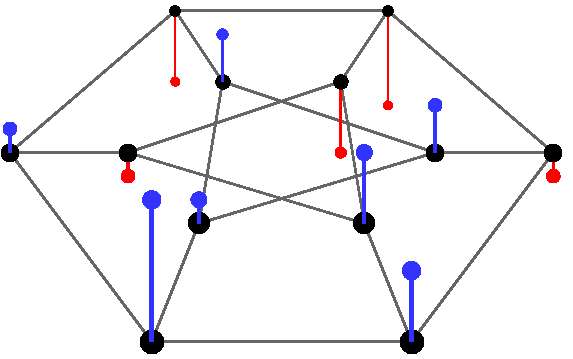
\includegraphics[width=0.35\linewidth]{Figures/signal_duher_graph_2.pdf}
	\floatsource
	\label{fig:duher}
\end{figure}

\subsection{The challenge of graph-like domains}

One of the reasons why GSP has been such a fertile field, allowing the birth of so many different problems and ideas, is that the definition of a signal over a graph leads to a series of obstacles when attempting to use even the most fundamental concepts of signal processing. Let us take the simple but elucidating example given by Shuman \emph{et al.}~\cite{shuman2013emerging}, and consider the unit shift to the right of a discrete-time signal $ x[n] $, which is done in digital signal processing by the simple variable substitution $ x[n-1] $. Good enough, but what does it mean to right-shift the signal in  Fig. \ref{fig:duher}, for example? Obviously the sense of right and left are meaningless for general graphs. On this problem, Shuman \emph{et al.} argue that a na\"ive choice would be to label the $ N $ graph vertices from $ v_0 $ to $ v_{N-1} $, so that the sample $ x[n] $ is assigned to vertex $ v_n $, for doing so would allow to define the shifted signal as the result of assigning $ x[n] $ to vertex $ v_{(n-1) \text{\,mod\,} N} $. Such an option, however, is not adequate, for its repeatability depends always on the way the vertices are labeled. This example illustrates how a concept in DSP as simple as signal translation may deserve a cautious study in GSP.


\section{Principles and definitions}
\label{sec:II}
The field of graph signal processing draws basic concepts from the classical theories of digital signal processing and graph theory, aiming to provide a cohesive and useful framework to tackle the aforementioned challenges. In this section, some of the main definitions found in this field are presented.


\subsection{Graph theory: a brief terminology}

A graph is commonly defined as the ordered pair  $ (\mathcal{V},\mathcal{E}) $, in which the set $ \mathcal{V} $ contains the so called graph \emph{vertices} and the set of \emph{edges} $ \mathcal{E} $ is a subset of $ \mathcal{V}^2 $ \cite{feofiloff2011introduccao}.  We will usually indicate by $ |\mathcal{V}| = N $\footnote{The set operator $ |\cdot| $ means the cardinality, or amount of elements, of the set.} and $ |\mathcal{E}| = E $ the number of vertices and edges of a graph, respectively. For our purposes it is convenient to represent a graph as the structure $ \mathcal{G} = \{\mathcal{V}, \mathbf{A}\} $, endowed with the (weighted) adjacency matrix $ \mathbf{A} $ which captures the vertex-to-vertex relations: if $ A_{i,j} \neq 0$, then there is an edge of weight $ A_{i,j} $ from the vertex $ v_j $ to $ v_i $. It is denoted by $ d_i^- $ the \emph{indegree} of vertex $ v_i $, consisting of the sum of weights of all incoming edges to vertex $ v_i $. Likewise, the \emph{outdegree} $ d^+_i $ is the sum of weights of edges departing from $ v_i $.

A graph is called \emph{undirected} if and only if its adjacency matrix is symmetric, in which case it is defined the \emph{degree} of vertex $ v_i $ as $ d_i^- = d_i^+ = d_i $. In this case, a graph is said to be \emph{d-regular} whenever all graph vertices have degree $ d $\label{pag:regular}. If $ \mathbf{A} $ is asymmetric, however, the respective graph is \emph{directed} and its pictorial representation depicts the edges as arrows, to account for the unidirectional relation between adjacent vertices. Examples of directed and undirected graphs are shown in Fig. \ref{fig:example_graphs}.

\begin{figure}
	\centering
    \caption{Examples of (a) directed and (b) undirected graphs, defined over the same vertex set.}
	\subfloat[]{
		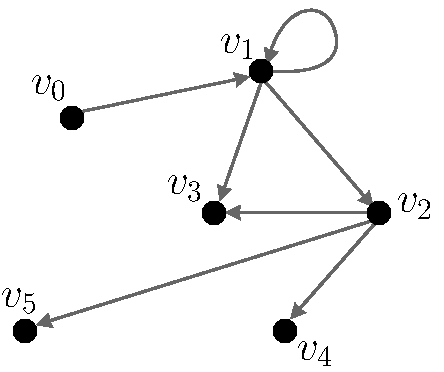
\includegraphics[width=0.25\linewidth]{Figures/example_graph_01_math.pdf}
	}~
	\subfloat[\label{fig:example_graphs_b}]{
		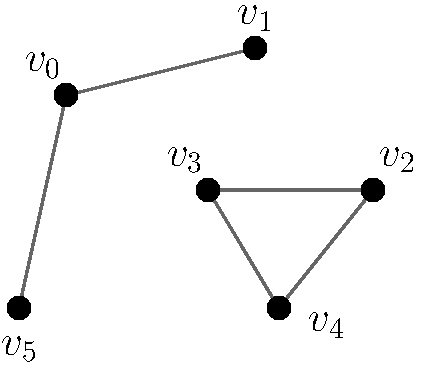
\includegraphics[width=0.25\linewidth]{Figures/example_graph_02_math.pdf}
	}
	\floatsource
	\label{fig:example_graphs}
\end{figure}

The adjacency matrix is the building block for one of the two main frameworks of GSP, what will be covered soon, but another matrix of great importance, mainly in the branch of GSP originated from spectral graph theory, is the Laplacian matrix
\begin{equation}
%\label{key}
\mathbf{L} = \mathbf{D} - \mathbf{A},
\end{equation}
with the \emph{degree matrix} $ \mathbf{D} $ being a diagonal matrix with $ d_i $ as the $ i $-th entry of its main diagonal. Depending on the context, $ \mathbf{D} $ may be taken as the indegree or outdegree matrix, although when the Laplacian matrix is used the graphs considered are often undirected.

A \emph{path} is a set of distinct edges (with the same orientation, if the graph is directed) linking distinct vertices, so that one could traverse all vertices by walking over the edges without ever repeat an edge or a vertex. A \emph{cycle} is like a path, except that it has equal starting and end vertices, and if a graph has a cycle it is called \emph{cyclic} (\emph{acyclic}, otherwise). If the cycle has only one edge, it is called a \emph{loop}. One refers to \emph{multiple edges} whenever a single pair of vertices is connected by two or more edges. An undirected graph is called \emph{simple} if it has no loops nor multiple edges.

A graph is said to be \emph{complete} if any two of its vertices are adjacent. Graph signal processing over such graphs may be extremely cumbersome, for the computational complexity of many of its techniques depends heavily on the number of graph edges. For most applications, it is desirable to have a small number of edges while keeping the graph \emph{connected}, i.~e., for any pair of vertices there exists a path connecting them.

A graph is said to be \emph{unweighted} if all its edges have unit weight. A \emph{subgraph} of $ \mathcal{G} $ is a graph $ \mathcal{G}' = (\mathcal{V}', \mathbf{A}')$ with edge set $ \mathcal{E}' $, in which $ \mathcal{V}' \subset \mathcal{V} $ and $ \mathcal{E}' \subset \mathcal{E} $. A \emph{connected component} of $ \mathcal{G} $ is a connected subgraph $ \mathcal{G}' = (\mathcal{V}', \mathbf{A}')$ in which any vertex in $ \mathcal{V}' $ is linked exclusively to another vertex also in $ \mathcal{V}' $. This is illustrated by Fig. \ref{fig:example_graphs_b}, in which the graph has two connected components.

\begin{figure}
	\centering
    \caption{(a) A graph and (b) the set of vertices $ \mathcal{N}(i,2) $ shown in red, with $ v_i $ being depicted in white. The edges linking $ v_i $ to the elements in $ \mathcal{N}(i,2) $ are also highlighted in red.}%
	\subfloat[\label{fig:k_hop_neighborhood_01}]{
		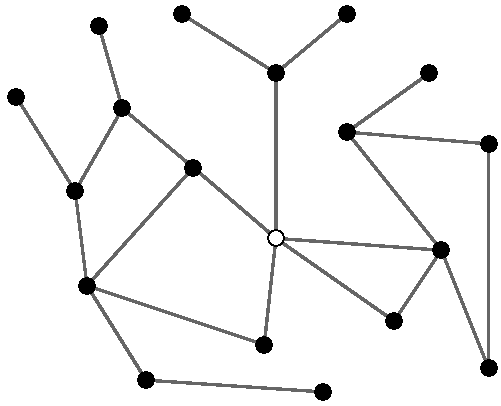
\includegraphics[width=0.25\linewidth]{Figures/k_hop_neighborhood_01.pdf}
	}~
	%	\qquad
	\subfloat[\label{fig:k_hop_neighborhood_02}]{
		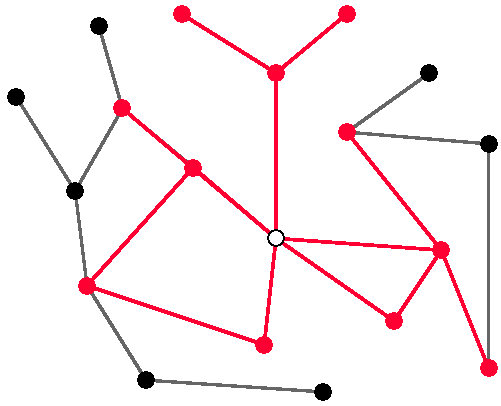
\includegraphics[width=0.25\linewidth]{Figures/k_hop_neighborhood_02.pdf}
	}
	%\hspace{0.2cm}%
	\floatsource
	\label{fig:k_hop_neighborhood}%
\end{figure}

The \emph{neighbourhood} of a vertex $ v_i $ is the set $ \mathcal{N}_i $ of all vertices adjacent to $ v_i $. Sometimes it is useful as well to denote by $ \mathcal{N}(i,K) $ the set of vertices connected to $ v_i $ through a path of length $ K $ or less. This notion is represented in Fig. \ref{fig:k_hop_neighborhood}.

The reader is encouraged to refer to this section whenever necessary. For a broader glossary with a solid introduction to graph theory, the reader may wish to read \cite{murty2008graph, chung1997spectral}.


\subsection{Defining a graph signal}

A signal $ \mathbf{s} $ defined over $ \mathcal{G} = \{\mathcal{V}, \mathbf{A}\} $, with $ |\mathcal{V}| = N $, is a discrete-domain function mapping the graph vertex set to a scalar set, usually the complex or real numbers,
\begin{equation}
\label{eq:def_signal}
s: \ \mathcal{V} \rightarrow \mathbb{C} \ | \ s(v_i) = s_i, \ i=0, \dots, N-1,
\end{equation}
so that the graph signal $ \mathbf{s} $ can be seen as a column vector in $ \mathbb{C}^N $ \emph{indexed by the vertices of} $ \mathcal{G} $. Once the vertices $ \mathcal{V} = \{v_1, \dots, v_N\}$ are clearly labeled, it is not ambiguous to represent the signal as the column vector $ \mathbf{s} = (s_0 \ s_1 \ \dots \ s_{N-1})^T$, $ s_i \in \mathbb{C} $, $ 0 \leq i \leq N-1 $.

\begin{figure*}
	\centering
    \caption{Examples of depictions of graph signals over (a) a directed ring graph,
		(b) an undirected regular grid graph and (c) a graph of cities from the Brazilian Northeastern region, over which was defined a signal of temperature measurements from February 1\textsuperscript{st} of 2012, retrieved from the
		\emph{Banco de Dados Meteorol\'ogicos para Ensino e Pesquisa} (BDMEP, freely translated as Meteorological Database for Teaching and Research), available at: \texttt{\url{http://www.inmet.gov.br/portal/index.php?r=bdmep/bdmep}}.}%
	\subfloat[\label{figa_graphs}]{
		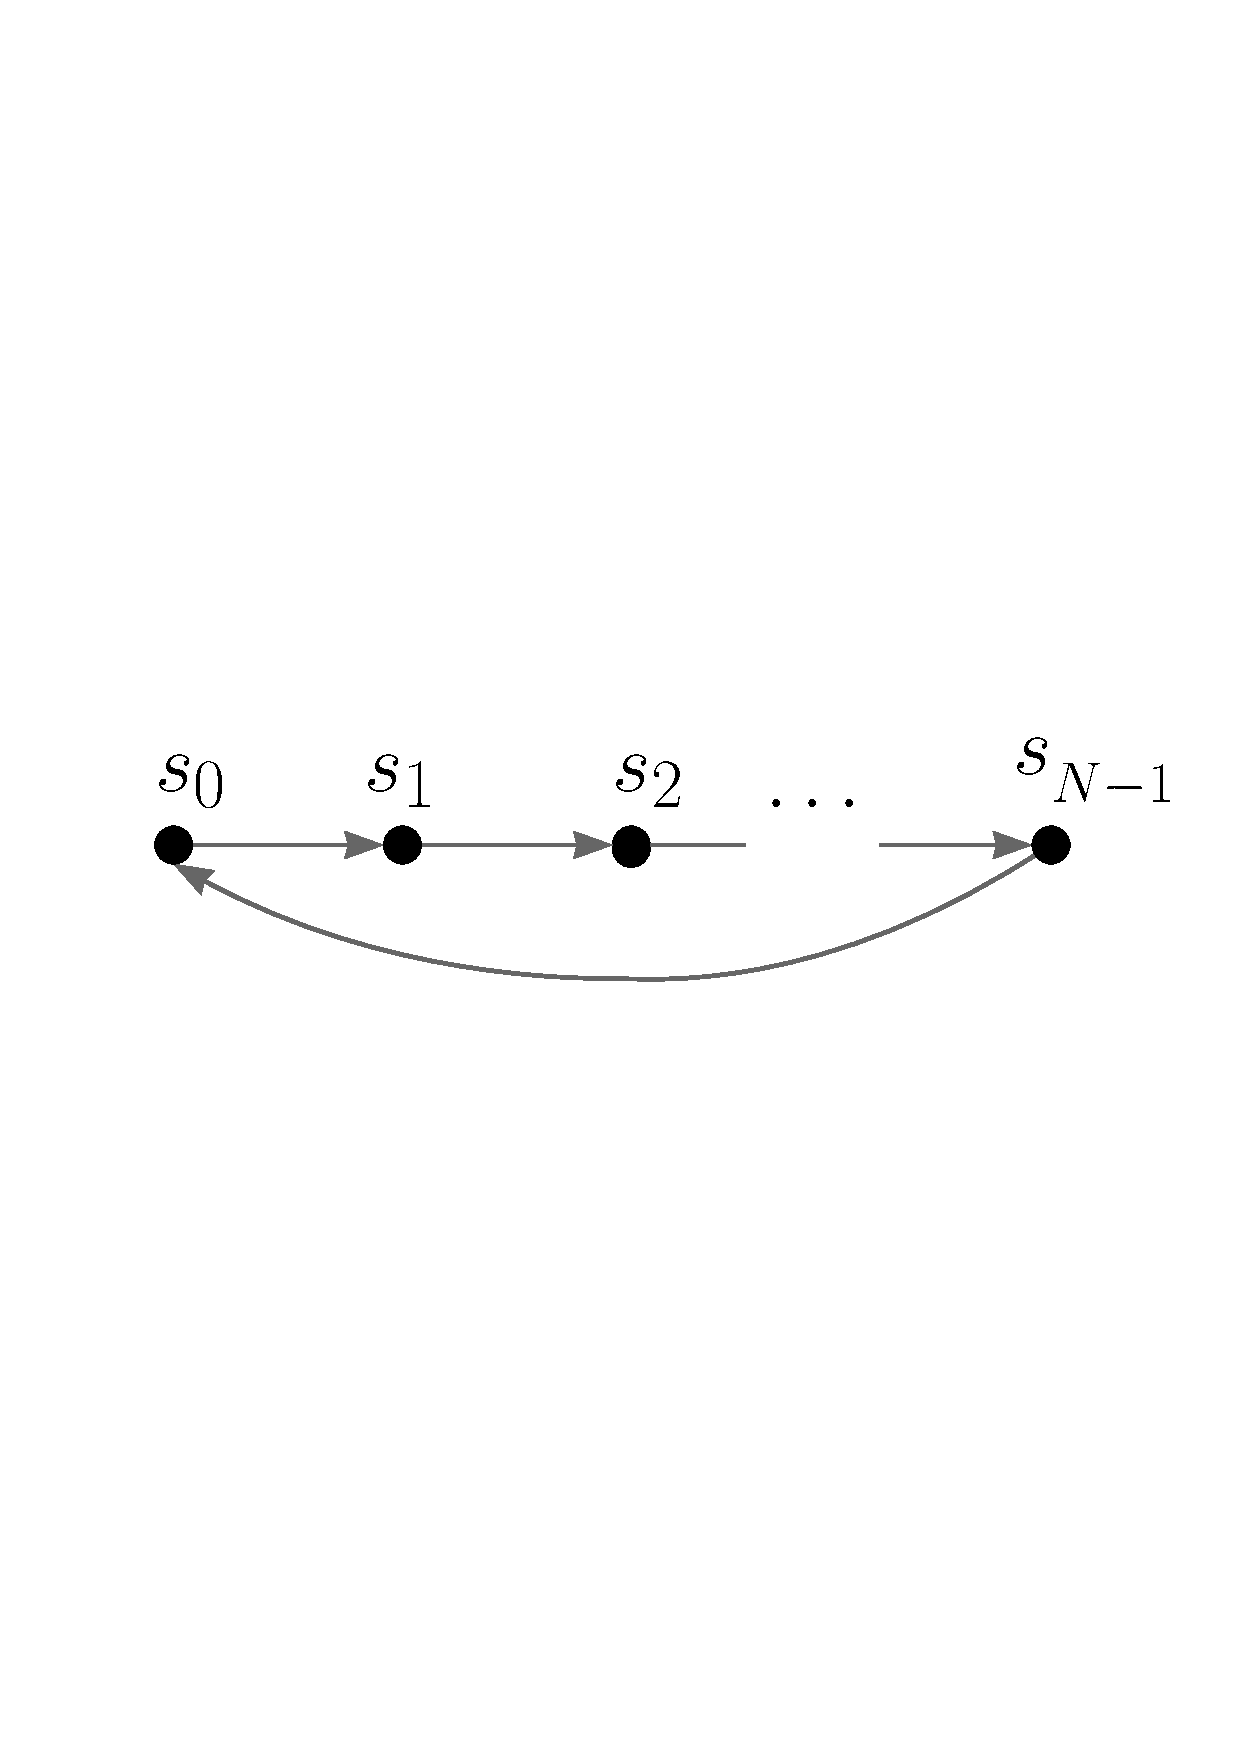
\includegraphics[width=0.25\linewidth]{Figures/signal_ring_graph_white_border.pdf}
	}
	\subfloat[\label{figb_graphs}]{
		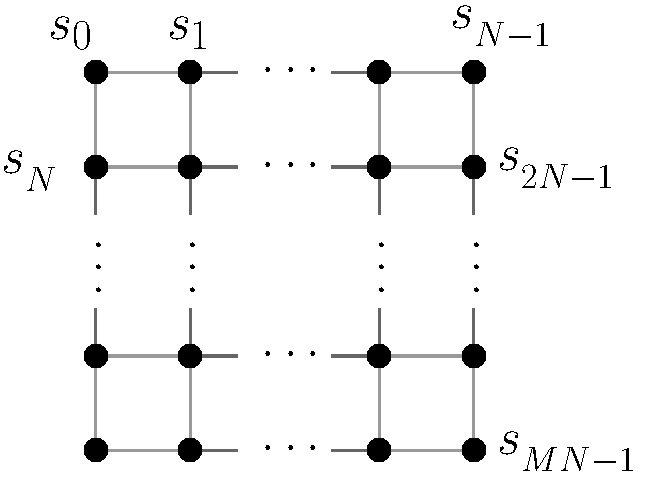
\includegraphics[width=0.25\linewidth]{Figures/image_graph.pdf}
	}%
	\subfloat[\label{figd_graphs}]{
		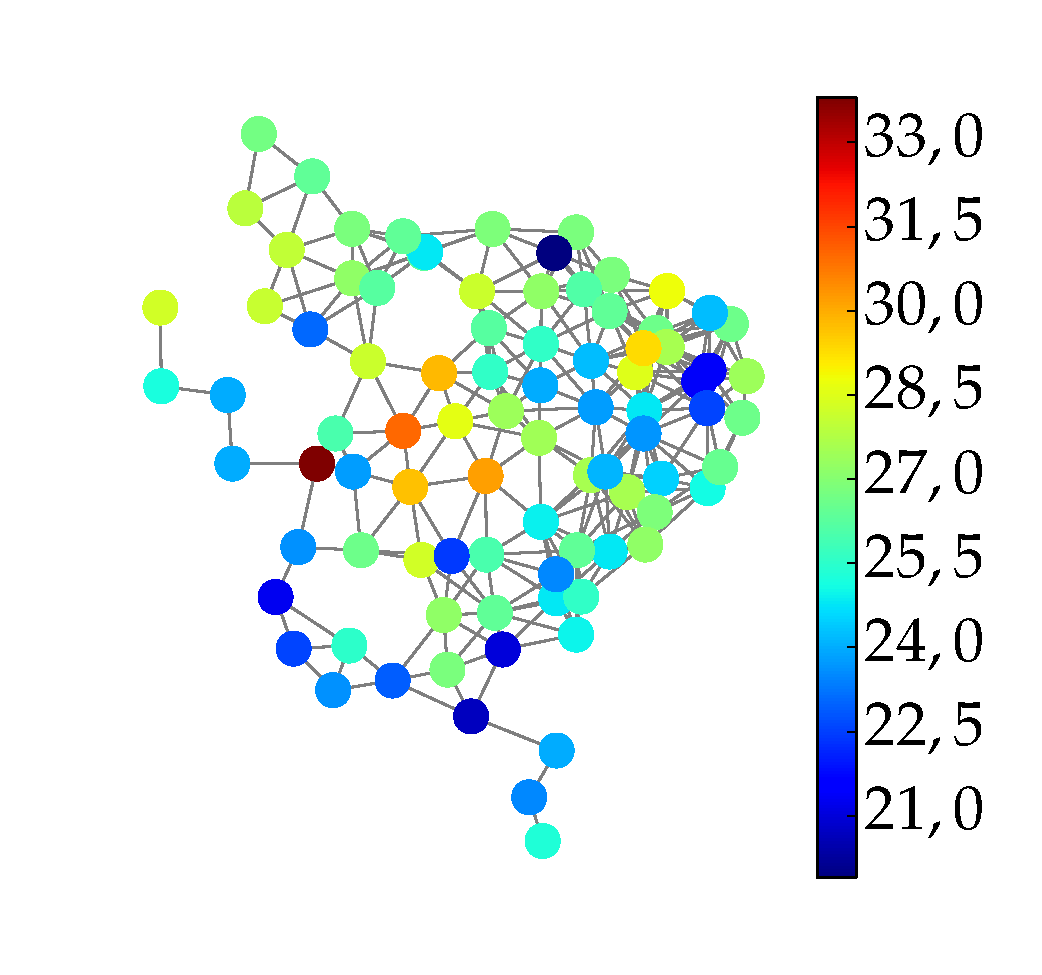
\includegraphics[width=0.3\linewidth]{Figures/temp_NE_stretched.pdf} }%
	\floatsource
	\label{fig:graphs}%
	\vspace{-0.2cm}
\end{figure*}

Fig. \ref{fig:graphs} provides examples of graph signal representations, in which the vertex labeling is omitted for the sake of simplicity, as it will be assumed that the signal sample $ s_i $ is assigned to vertex $ v_i $. The signal values are indicated in two manners: either by writing down its numerical value next to the respective vertex, or by using a pseudocolor scale, the latter of which is the scheme adopted throughout this paper.

It is crucial to stress a certain graph which links GSP to the classical DSP theory: the directed ring graph, shown in Fig. \ref{figa_graphs}, which models the finite-length discrete-time domain. Its directed edges model the causality of time domain, whereas the feedback edge accounts for the boundary condition of periodicity imposed by the DFT analysis. Other signals that arise in practical applications have the respective graphs easily identified: the rectangular lattice in Fig. \ref{figb_graphs}, for example, models the digital image domain \cite{sandryhaila2012nearest}, and Fig. \ref{figd_graphs} shows an example of signal defined over a mesh network of sensors, with the edges weighted using the inverse of the euclidian distance, which arises in many scenarios such as IoT applications.

\begin{figure*}
	\centering
    \caption{The same signal defined over two similar graphs, one of them being (a) the undirected ring graph. In (b) and (d) are depicted the Fourier spectra of the signals in (a) and (c), respectively.}%
	\begin{minipage}[c]{0.24\linewidth}
		\subfloat[\label{fig:diff_struct_a}]{
			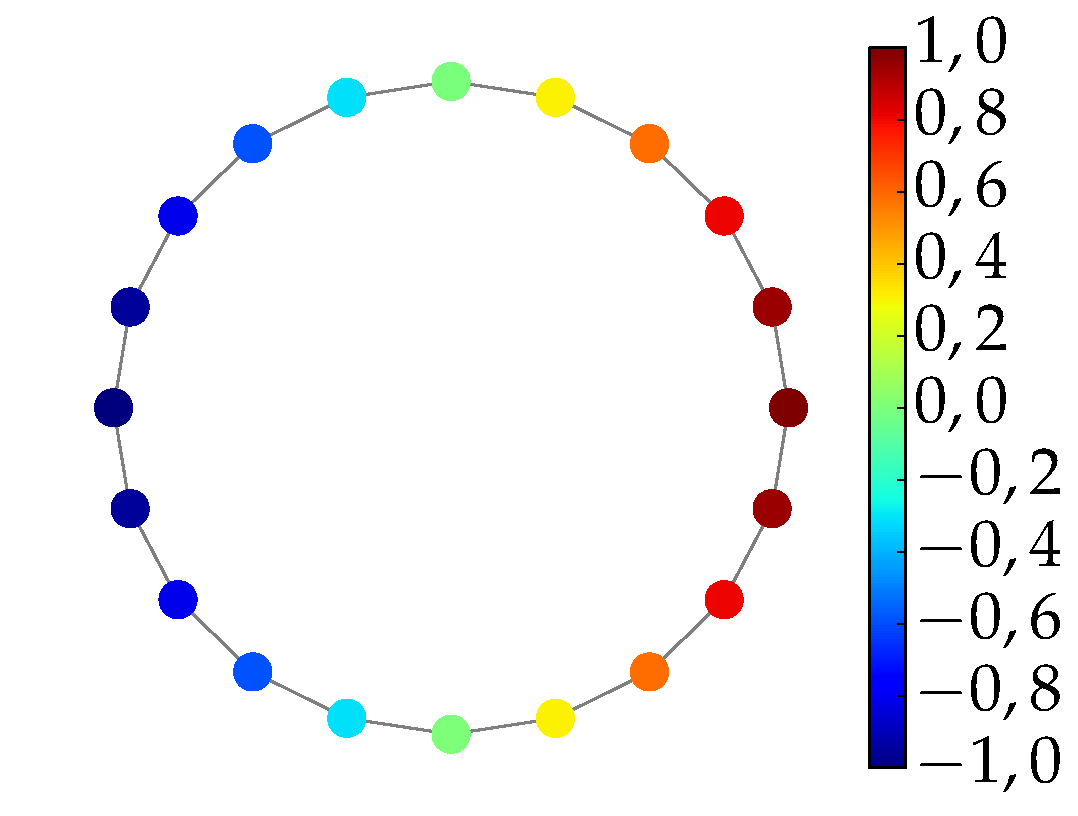
\includegraphics[width=\linewidth]{Figures/ring_different_structure_01.pdf}
		}
	\end{minipage} %
	\begin{minipage}[c]{0.24\linewidth}
		\subfloat[\label{fig:diff_struct_c}]{
			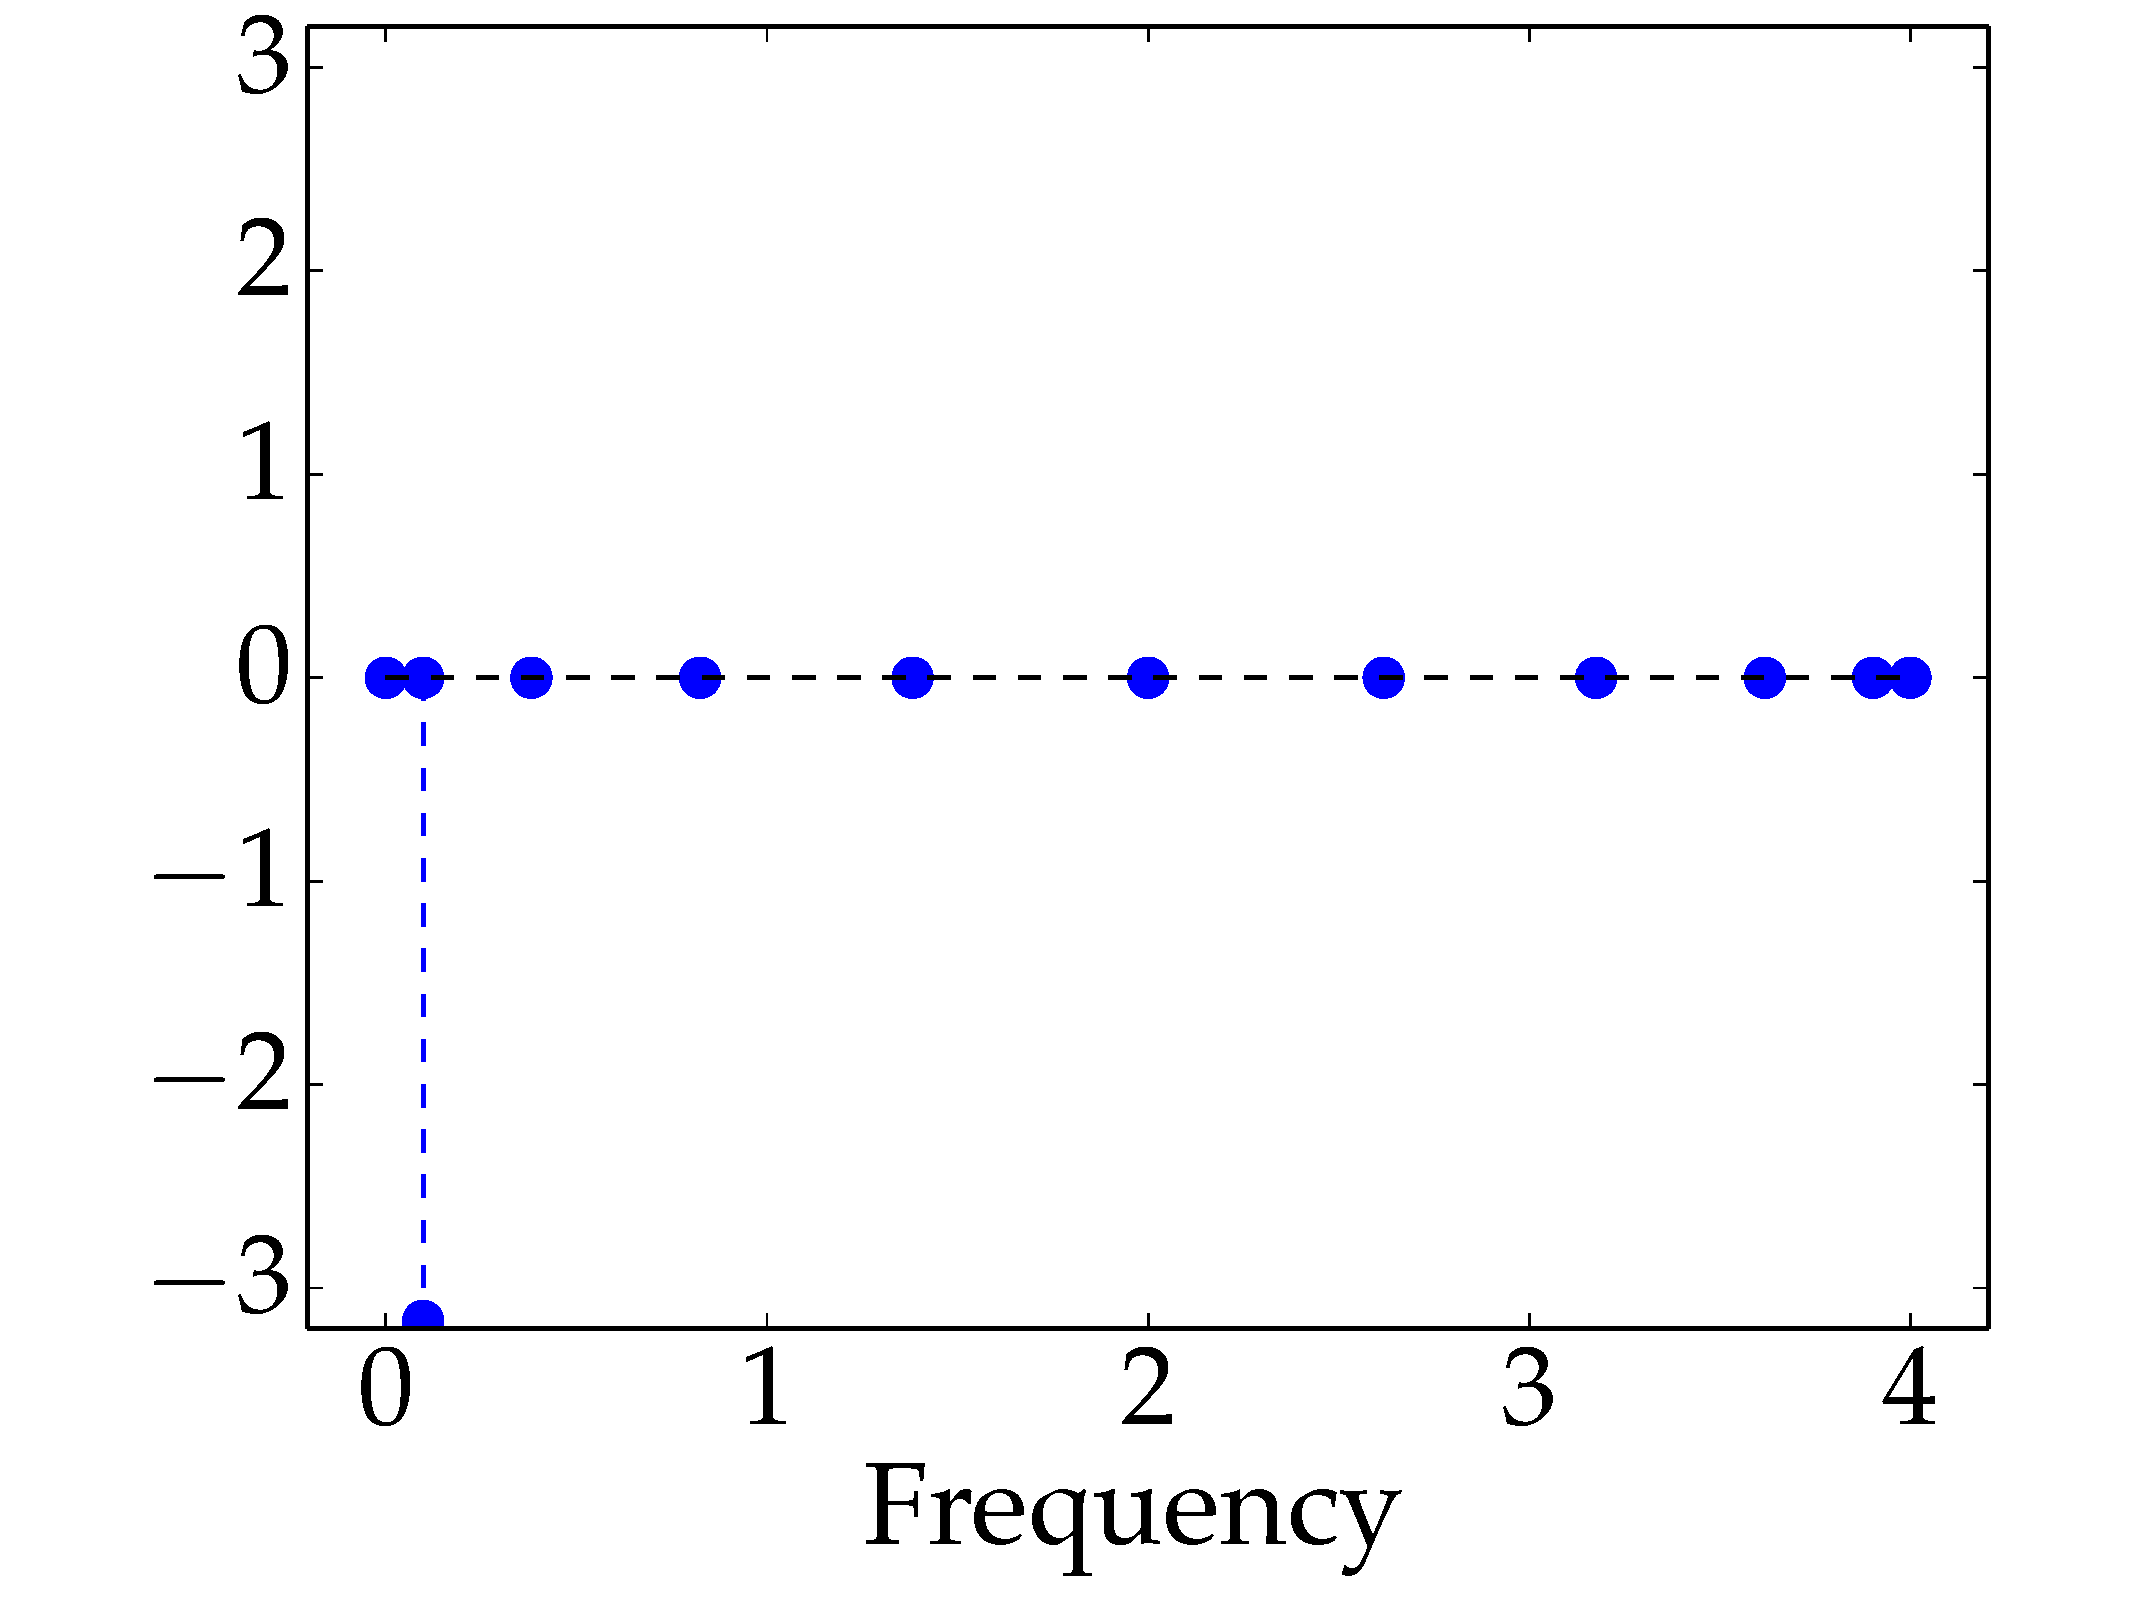
\includegraphics[width=\linewidth]{Figures/ring_different_structure_01_spectrum_EN.pdf}
		}
	\end{minipage}%
	\begin{minipage}[c]{0.24\linewidth}
		\subfloat[\label{fig:diff_struct_b}]{
			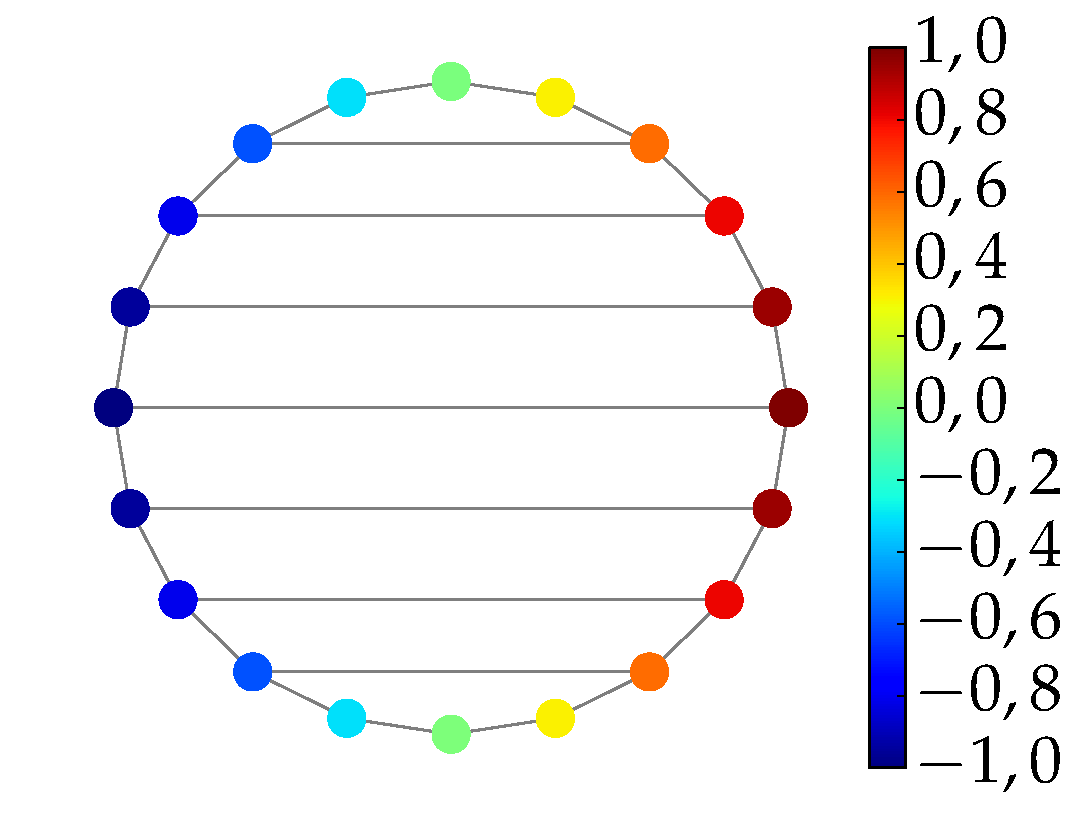
\includegraphics[width=\linewidth]{Figures/ring_different_structure_02.pdf}
		}~
	\end{minipage}%
	\begin{minipage}[c]{0.25\linewidth}
		\subfloat[\label{fig:diff_struct_d}]{
			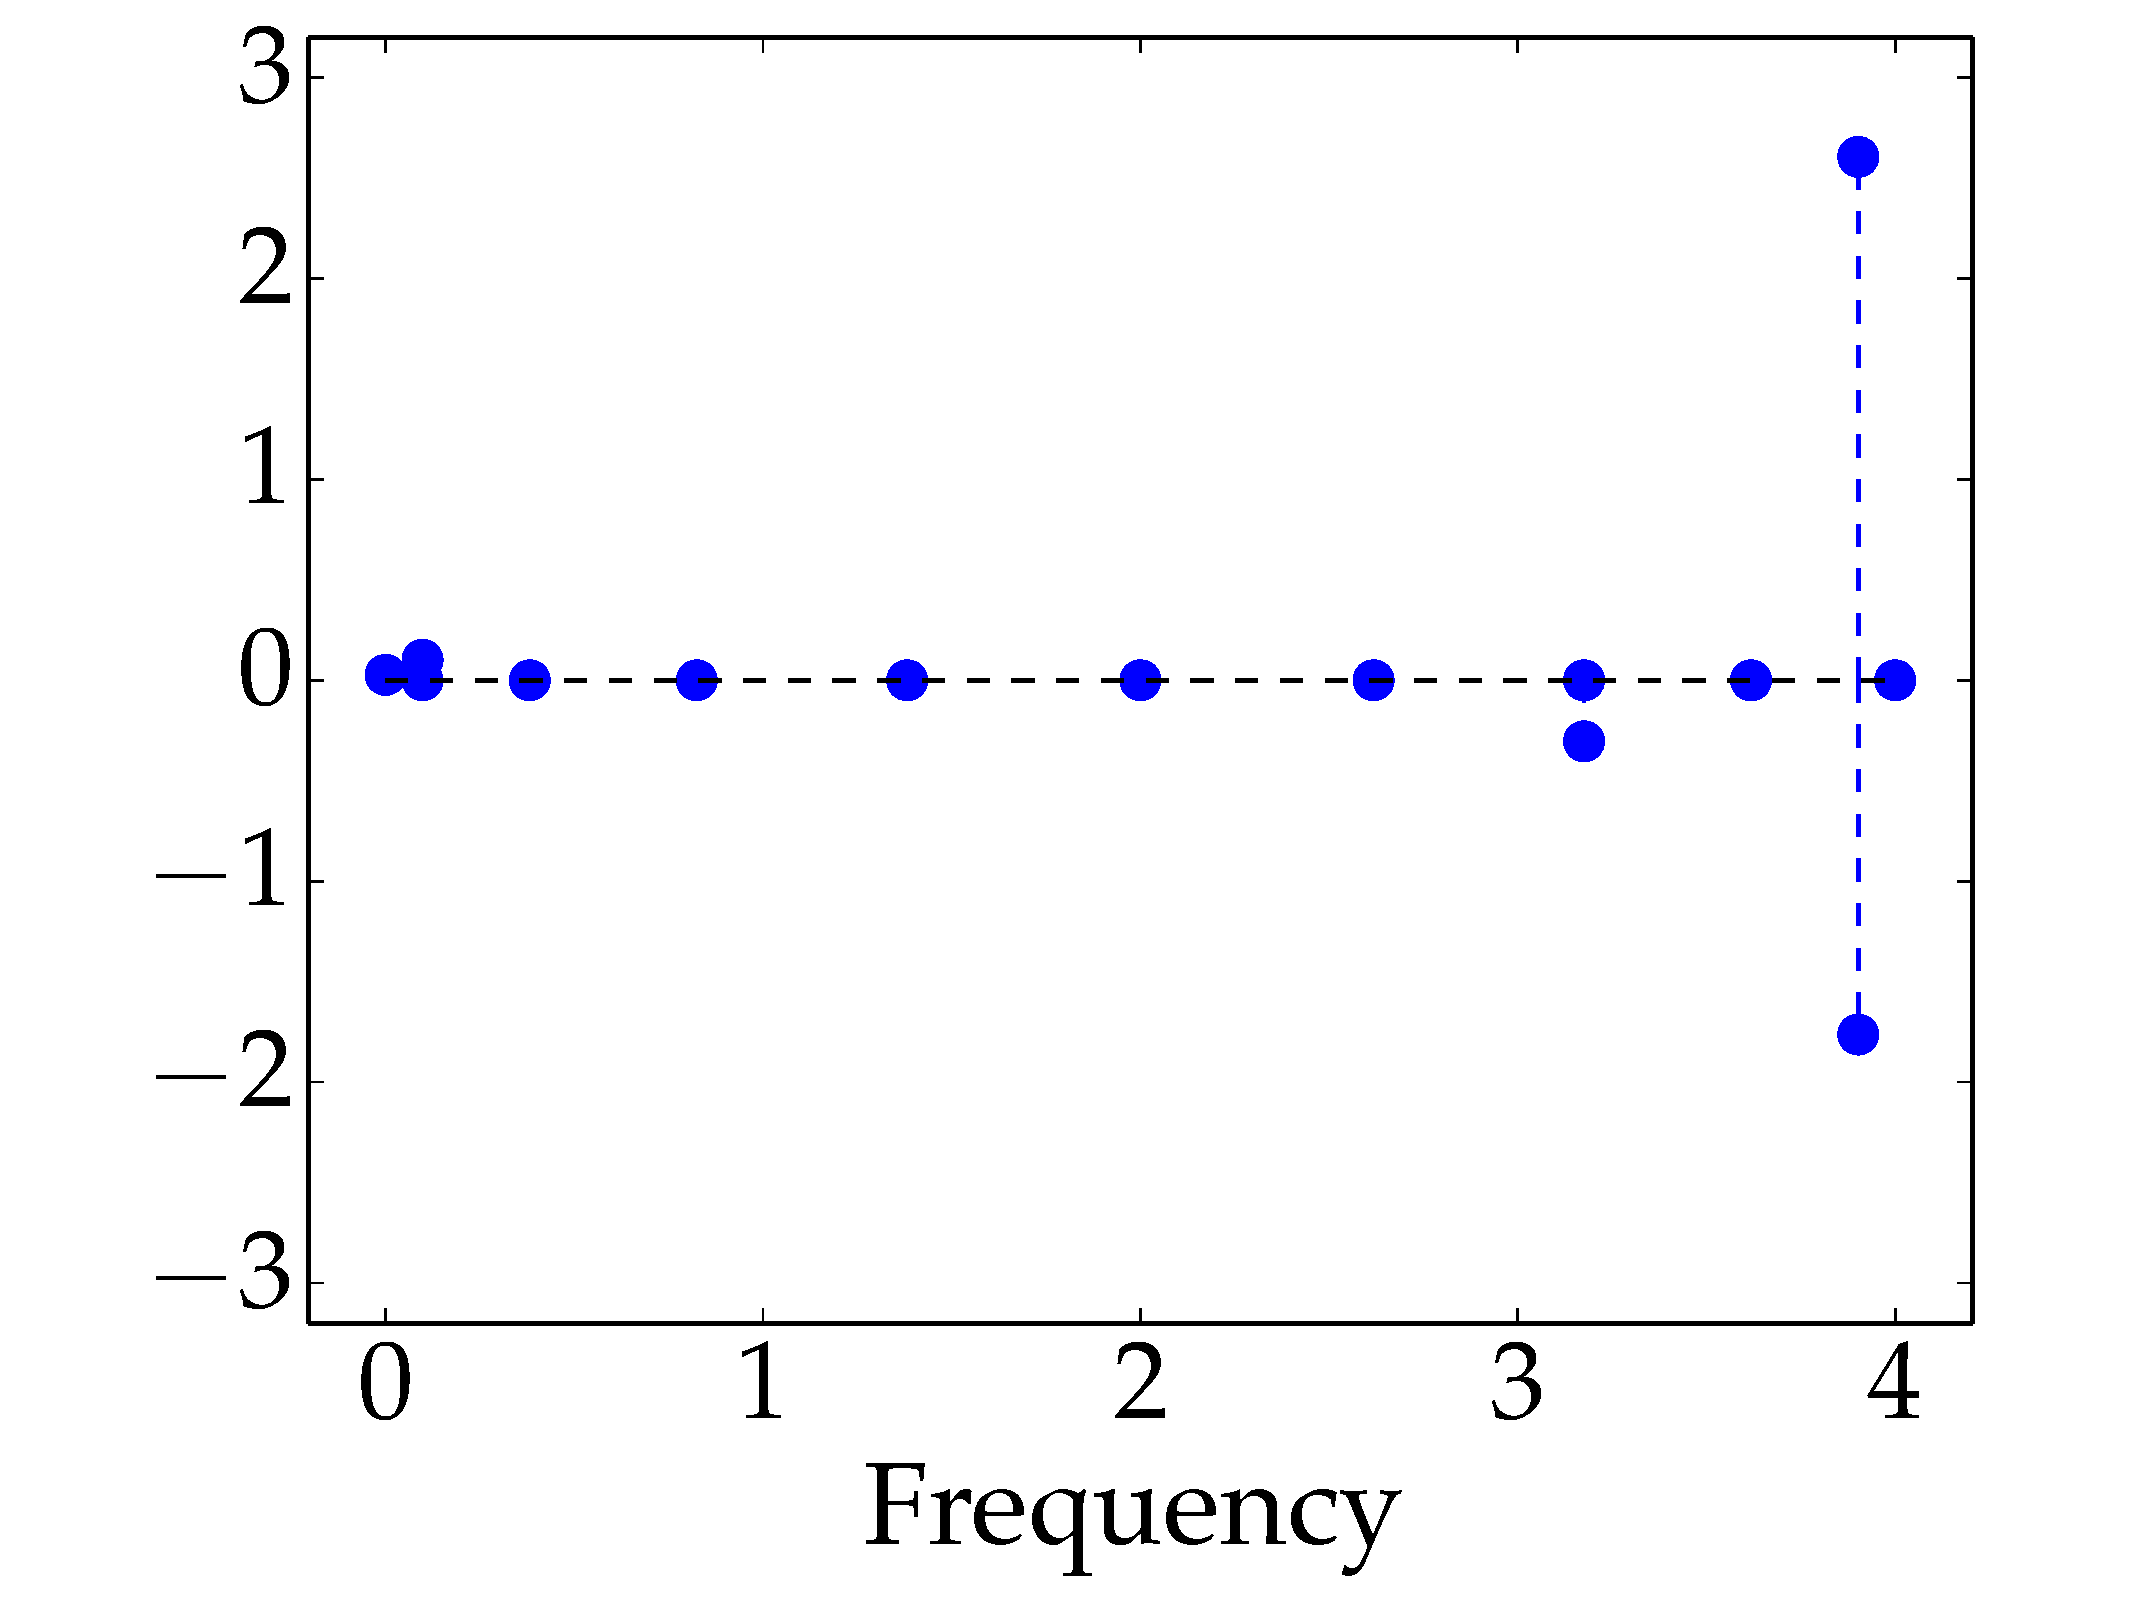
\includegraphics[width=\linewidth]{Figures/ring_different_structure_02_spectrum_EN.pdf}
		}
	\end{minipage}%
	\floatsource
	\label{fig:diff_struct}%
	\vspace{-0.2cm}
\end{figure*}

The spectral characteristics of a signal depend heavily on the domain over which it is defined, but one does not need to acknowledge this in the context of DSP, for in this case the domains are always regular and uniform.\footnote{One could argue that, in the theory of \emph{nonuniform sampling}, the signal is defined over an irregular domain, since the samples may be randomly spaced. Even in this case, however, the classical techniques still aim to \emph{recover} the signal so as to represent it in its usual -- and \emph{uniform} -- domain.
}
From the classical theory, the common understanding states that a signal has mostly low frequencies if adjacent samples have similar values, and high frequencies otherwise. When dealing with signals defined over graphs, it is clear that the adjacency relations depend on the graph topology, and therefore one may foresee that \emph{the same signal may present different spectra when defined over different graphs}. This intuition is visually confirmed (and will soon be mathematically proved) in Fig. \ref{fig:diff_struct}, which depicts a signal and its spectra\footnote{These spectra were obtained using the Laplacian matrix as a graph shift operator, not the adjacency matrix. The reader should not bother with the differences for now, it suffices to know that the spectra can be read as usual: frequencies increase as you move to the right on the frequency axis. In other words, any low-pass signal will have most of its energy lying on the left-hand side of the spectrum.} when two different graphs are taken as domain. The reader may notice that, in Fig. \ref{fig:diff_struct_b}, the samples with highest values are adjacent to the ones with small values, what causes the highest concentration of energy to be in the highest frequencies. The opposed behavior is observed in the signal defined over the undirected ring graph in Fig. \ref{fig:diff_struct_a}.

\subsection{Graph inference}
\label{subsec:inferindo}

Some contexts in which GSP is applied do not provide clear information on \emph{how the underlying graph is structured}. For example, let us suppose the temperature data (or any other data in fact) of some Brazilian Northeastern cities will be treated using GSP. How is one supposed to weight the graph edges, and before this, how does one decide which vertices to connect? Is the graph shown in Fig. \ref{figd_graphs} the only option? Clearly not. Although generally the problem of graph inference is complex, this type of geography-based graph has an adequate method of topology estimation.

The general ideia is that, if there is a clear metric to evaluate the \emph{expected} similarity between samples as a function of the available information regarding the respective vertices, then this metric may be used to generate the edge weight and a threshold is set so that any weight below this value causes the respective edge to be eliminated. In the case of vertices which have geographic location, the euclidian distance may be used as the metric because vertices that are closer together are (usually) \emph{expected} to have similar signal samples, and therefore the adjacency matrix of the underlying graph may have entries given by
\begin{equation}
\label{eq:weights}
A_{ij} =
\begin{cases}
\displaystyle
\exp \left(- \frac{\text{dist}^2(v_i, v_j)}{2 \theta^2}\right)& \text{ if } \text{dist}(v_i, v_j) < T \\ 
0 & \text{ otherwise},
\end{cases}
\end{equation}
as used in \cite{shuman2013emerging}. The choice of the parameters $ T $\footnote{$ T $ indicates a distance threshold above which we set the edge weight to zero, effectively leaving the vertices unlinked. This means that the distance between them is assumed to be too high for any significant interdependence to exist.} and $ \theta $ (standard deviation of the distribution), and of how to use the metric (in this case, inside a Gaussian distribution), are dictated by the application and by the analyst experience. 

However, if there is an isolated vertex, far from the others, the use of (\ref{eq:weights}) may lead to a compromise between keeping the graph connected and obtaining a sparse adjacency matrix, since imposing connectivity to the graph in this case implies increasing $ T $, and therefore having many edges. To deal with this problem and still have a good representation of the underlying graph, one alternative is to connect a vertex to its $ K $ closest neighbours (setting $ K $ to an appropriate value, according to the context) and weight the edges using the Gaussian distribution in (\ref{eq:weights}).

As previously discussed, these methods require an adequate metric to evaluate the expected similarity between samples in the graph vertex, but given the diverse areas in which graph signals may arise, estimating the topology of the  underlying graph constitutes a challenge of its own \cite{mei2016signal,Sardellitti2016}.

\section{Formulating GSP based on the graph adjacency matrix}
\label{sec:DSPG}

In 2008, P\"uschel and Moura published their \emph{algebraic signal processing} (ASP) theory \cite{puschel2008time,puschel2008space}, which expands DSP by looking at it from an algebraic point of view: each signal processing theory is studied as a triple $ (\mathscr{A}, \mathscr{M}, \Phi) $ consisting of an algebra $ \mathscr{A} $ (a vector space endowed with multiplication between vectors), an $ \mathscr{A} $-module $ \mathscr{M} $ (a vector space over the same base field as $ \mathscr{A} $ which admits left-multiplication by elements of $ \mathscr{A} $) and a linear transformation $ \Phi $. $ \mathscr{A} $ is called the filter space, $ \mathscr{M} $ is the signal space and $ \Phi $ is the Fourier transform (homomorphism over $ \mathscr{M} $) associated with the structure.

When these authors drew inspiration from ASP to develop their GSP theory, the starting point was necessarily to find (better, to define) the unit shift operator of graph signals, the reason being that such an operator in ASP is the building block of the algebra $ \mathscr{A} $ (as, for example, the unit delay $ z^{-1} $ is the building block for filters of discrete-time and finite-length signals $ \mathscr{A}  = \{ \sum_{\ell=0}^{N-1} h_\ell z^{-\ell} | h_\ell \in \mathbb{C} \}$). To do so, the shift of discrete-time signals, defined over directed ring graphs, was investigated.

By inspection of the \emph{adjacency matrix} of the directed ring graph (Fig. \ref{figa_graphs}),
\begin{equation}\label{eq:C}
\mathbf{C} =
\begin{bmatrix}
&  &  &   1\\ 
1 &  &   & \\ 
&   \ddots &  & \\ 
&  &   1 & 
\end{bmatrix},
\end{equation}
it was noticed that the unit (circular) shift of discrete-time signals is precisely the left-multiplication by $ \mathbf{C} $, for a given discrete-time signal $ \mathbf{x} = (x_0 \ x_1 \ \dots \ x_{N-1})^T $,
\begin{equation}\label{eq:unit_shift}
\mathbf{C}\mathbf{x} =
\begin{bmatrix}
&  &  &   1\\ 
1 &  &   & \\ 
&   \ddots &  & \\ 
&  &   1 & 
\end{bmatrix}
\begin{bmatrix}
x_0 \\ x_1 \\ \vdots \\ x_{N-1}
\end{bmatrix} =
\begin{bmatrix}
x_{N-1} \\ x_0 \\ \vdots \\ x_{N-2}
\end{bmatrix} \overset{\Delta}{=} \mathbf{x}^{\langle 1 \rangle},
\end{equation}
and the generalization followed: \emph{the graph unit shift was defined as the left-multiplication by the graph adjacency matrix}.

In other words, for a signal $ \mathbf{x} $ defined over the graph $ \mathcal{G} = \{\mathcal{V}, \mathbf{A}\} $, the adjacency matrix $ \mathbf{A} $ acts as a \emph{filter} which ``delays'' (i.~e., translates in the vertex domain) the graph signal $ \mathbf{x} $ (represented here as a column vector) by one unit, producing the delayed version represented hereinafter by $ \mathbf{x}^{\langle 1 \rangle} = \mathbf{A} \mathbf{x}$.

\subsection{Graph filters}
\label{subsec:filtros}

Seeing the adjacency matrix as a filter suggested the general definition of \emph{graph filter} as any matrix $ \mathbf{H} \in \mathbb{C}^{N \times N} $ \cite{sandryhaila2013filters}, which preserves the necessary property that the output of a filter (i.~e., the matrix-vector product) is a signal (i.~e., a column vector). Such a definition implies that \emph{linearity} is always valid for graph filters, since the distributivity of matrix multiplication with respect to matrix addition guarantees that
\begin{equation}
%\label{key}
\mathbf{H} (\alpha_1 \mathbf{x}_1 + \alpha_2 \mathbf{x}_2) =  \alpha_1 \mathbf{H} \mathbf{x}_1 + \alpha_2 \mathbf{H}  \mathbf{x}_2.
\end{equation}

The next desirable property would be \emph{shift invariance}, analogous to the classical time invariance of DSP, and this means that filtering and shifting should commute. In other words, for a graph filter $ \mathbf{H} $ to be \emph{linear and shift invariant} (LSI) it is required that
\begin{equation}
\label{eq:lsi_def}
\mathbf{A} \mathbf{H} \mathbf{x} = \mathbf{H} \mathbf{A} \mathbf{x}, \ \ \forall \mathbf{x} \in \mathbb{C}^N
\Rightarrow
\mathbf{A} \mathbf{H} = \mathbf{H} \mathbf{A}.
\end{equation}
% $ \mathbf{A} \mathbf{H} \mathbf{x} = \mathbf{H} \mathbf{A} \mathbf{x} \ \forall \mathbf{x}$, and therefore $ \mathbf{A} \mathbf{H} = \mathbf{H} \mathbf{A}$.
% Sandryhaila and Moura have shown \cite{sandryhaila2013discrete,sandryhaila2014big} that LSI filters can be represented as polynomials $ h(\cdot) $ evaluated over $ \mathbf{A} $,
% \begin{equation}
% \label{eq:filter_poly}
% h(\mathbf{A}) = \sum_{\ell=0}^{L-1} h_\ell \mathbf{A}^\ell,
% \end{equation}
% with $ L $ smaller than or equal to the degree of the minimal polynomial of $ \mathbf{A} $, i.~e., LSI filters are finite power series on the shift operator, exactly as it happens in DSP, in which LTI filters have polynomial representations on $ z^{-1} $.
The following theorem establishes an important property satisfied by every LSI filter~\cite{sandryhaila2013discrete} .
\vspace{0.2cm}
\begin{theorem}
\label{theo:01}
Let $ \mathbf{A} $ be the adjacency matrix of a graph. Let us assume that the characteristic polynomial $char_{\mathbf{A}}(x)$ of $\mathbf{A}$ coincides with the respective minimal polynomial $m_{\mathbf{A}}(x) $. Therefore, $ \mathbf{H} $ is an LSI filter if and only if $ \mathbf{H} $ is a polynomial in $ \mathbf{A} $, i.~e.
\begin{equation}\label{eq:filtro}
\mathbf{H} = h(\mathbf{A}) = \sum_{\ell=0}^{L} h_\ell \mathbf{A}^\ell,
\end{equation}
where $ \mathbf{A}^0 $ is the identity matrix and $ L < \deg(m_{\mathbf{A}}) $.
\end{theorem}

The assumption on $char_{\mathbf{A}}(x)$ and $m_{\mathbf{A}}(x)$ in Theorem~\ref{theo:01} does not hold for all adjacency matrices $\mathbf{A}$. Nevertheless, the result in the referred theorem can be extended to all matrices using the concept of \emph{equivalent graph filters}, as clearly explained in~\cite{sandryhaila2013filters}. As a consequence, for any graph $\mathcal{G} = \{\mathbf{A}, \mathcal{V}\}$, every LSI filter has polynomial representation in $\mathbf{A}$. In this sense, Theorem~\ref{theo:01} suggests a convenient analogy with the classical DSP, since every filter for discrete-time signals can be represented as polynomials evaluated in $ z^{-1} $, the unit delay, via the $z$-transform of its impulse response.

\subsection{Graph Fourier transform}

The topic of spectral analysis is key in signal processing. When studying how this would be implemented in the scope of GSP, the authors started by looking at the classical Fourier transform as a signal decomposition into a basis of eigenfunctions of the LTI filtering \cite{oppenheim1997signals}, i.~e., the basis of complex time exponentials. From that point, the generalization to GSP was clear: the \emph{graph Fourier transform} (GFT) was defined as the decomposition of a graph signal into a basis of eigenvectors of LSI filtering.\footnote{One may wish to distinguish between the different implementations of the GFT regarding the choice of graph shift operator. Unless clearly stated otherwise, this chapter considers it to be always the graph adjacency matrix, but other popular option is the graph Laplacian, as already mentioned. In this regard, the reader even may find the terms GSP\textsubscript{A} and GSP\textsubscript{L} in previous publications \cite{ribeiro2018}, making the distinction clear.}

Let us take the graph $ \mathcal{G} = \{\mathcal{V}, \mathbf{A}\} $, $ |\mathcal{V}| =N $. If $ \mathbf{A} $ is diagonalizable,\footnote{If not, the reasoning may be replicated using the Jordan decomposition of $ \mathbf{A} $ and the set of generalized eigenvectors \cite{deri2017spectral}.} then one may write
\begin{equation}\label{eq:gft_01}
\mathbf{A} = \mathbf{V} \mathbf{\Lambda} \mathbf{V}^{-1},
\end{equation}
in which $ \mathbf{V} $ contains the $ N $ eigenvectors of $ \mathbf{A} $ in its columns,
\begin{equation}\label{eq:gft_02}
\mathbf{V} = (\mathbf{v}_0 \ \mathbf{v}_1 \ \dots\ \mathbf{v}_{N-1}).
\end{equation}

Since LSI filters are polynomials in $ \mathbf{A} $, and since a matrix and its powers share the same set of eigenvectors, the columns of $ \mathbf{V} $ form a basis of vectors invariant to LSI filtering. Besides, given that the subspaces generated by the linearly independent eigenvectors of a same eigenvalue of $ \mathbf{A} $ are irreducible, have null intersection and the dimensions of all subspaces add to $ N $ \cite{sandryhaila2013gft}, $ \mathbf{V} $ provides a basis which is invariant to LSI filtering for the space of signals defined over $ \mathcal{G} $.

Therefore, a signal $ \mathbf{x} $ may be decomposed into its components with respect to $ \mathbf{V} $ as
\begin{align}\label{eq:GFT_inv}
\mathbf{x} &= \widehat{x}_0 \mathbf{v}_0 + \dots + \widehat{x}_{N-1} \mathbf{v}_{N-1} \notag \\
&= \mathbf{V} (\widehat{x}_0 \ \widehat{x}_1 \ \dots \ \widehat{x}_{N-1})^T \notag \\
&= \mathbf{V} \widehat{\mathbf{x}} \overset{\Delta}{=} \textrm{GFT}\{\mathbf{x}\},
\end{align}
and this is the synthesis equation of the GFT. The analysis equation follows,
\begin{equation}\label{eq:GFT_fwd}
\widehat{\mathbf{x}} = \mathbf{V}^{-1} \mathbf{x} \overset{\Delta}{=} \textrm{GFT}^{-1}\{\mathbf{x}\}.
\end{equation}

It has been emphasized that the directed ring graph is the link between GSP and DSP, because it models the discrete-time domain. This provides a way of checking how consistent with the classical theory are the proposed GSP tools. When investigating how the GFT would act upon discrete-time signals, one should first diagonalize the adjacency matrix $ \mathbf{C} $ of the directed ring graph, given by (\ref{eq:C}). Since it is circulant, it is known to be diagonalized by the DFT matrix $ \mathbf{F} $, with entries $ F_{n,k} = \exp \left( -j\frac{2 \pi}{N} nk \right) $, which contains in its \emph{rows} the DFT eigenvectors. The calculation of the characteristic polynomial of $ \mathbf{C} $,
\begin{equation}
%\label{key}
p_{\mathbf{C}}(\lambda) = \text{det} (\lambda \mathbf{I} - \mathbf{C}) =
\begin{vmatrix}
\lambda &  &  &   -1\\ 
-1 & \lambda &   & \\ 
&   \ddots & \ddots & \\ 
&  &   -1 & \lambda
\end{vmatrix}
=\lambda^N - 1,
\end{equation}
shows that its eigenvalues are the $ N $ complex roots of unity. Setting these eigenvalues as the entries of a diagonal matrix $ \mathbf{\Lambda}_{\mathbf{C}} $, the eigendecomposition of $ \mathbf{C} $ may be written as
\begin{equation}\label{eq:diag_C}
\mathbf{C} = \mathbf{F}^{-1} \mathbf{\Lambda}_{\mathbf{C}} \mathbf{F},
\end{equation}
and one can see that, in the case of directed ring graphs, the GFT and the DFT matrices \emph{coincide}, since $ \mathbf{V}^{-1} = \mathbf{F} $. This equivalence indicates a desirable consistency with the classical theory.

 \subsection{The frequency domain}

The way the GFT was defined naturally suggests the interpretation of the adjacency matrix eigenvectors $ \mathbf{v}_i $ as ``frequency components'' associated with the ``graph frequencies'' given by the eigenvalues $ \lambda_i $, exactly as the Fourier component $ e^{-\qi \Omega t} $, in the continuous time domain $ t $, is associated with the frequency $ \Omega $. This subsection aims to provide the mathematical justification used by Sandryhaila and Moura \cite{sandryhaila2014frequency} to support this understanding, along with some authorial comments.

\begin{figure}
	\centering
    \caption{(a) Signal defined over an undirected ring graph and (b) its spectrum. The frequencies are indicated by the eigenvalues of the adjacency matrix.}%
	\begin{minipage}[c]{0.25\linewidth}
		\subfloat[\label{fig:diff_struct_a_GSPA}]{
			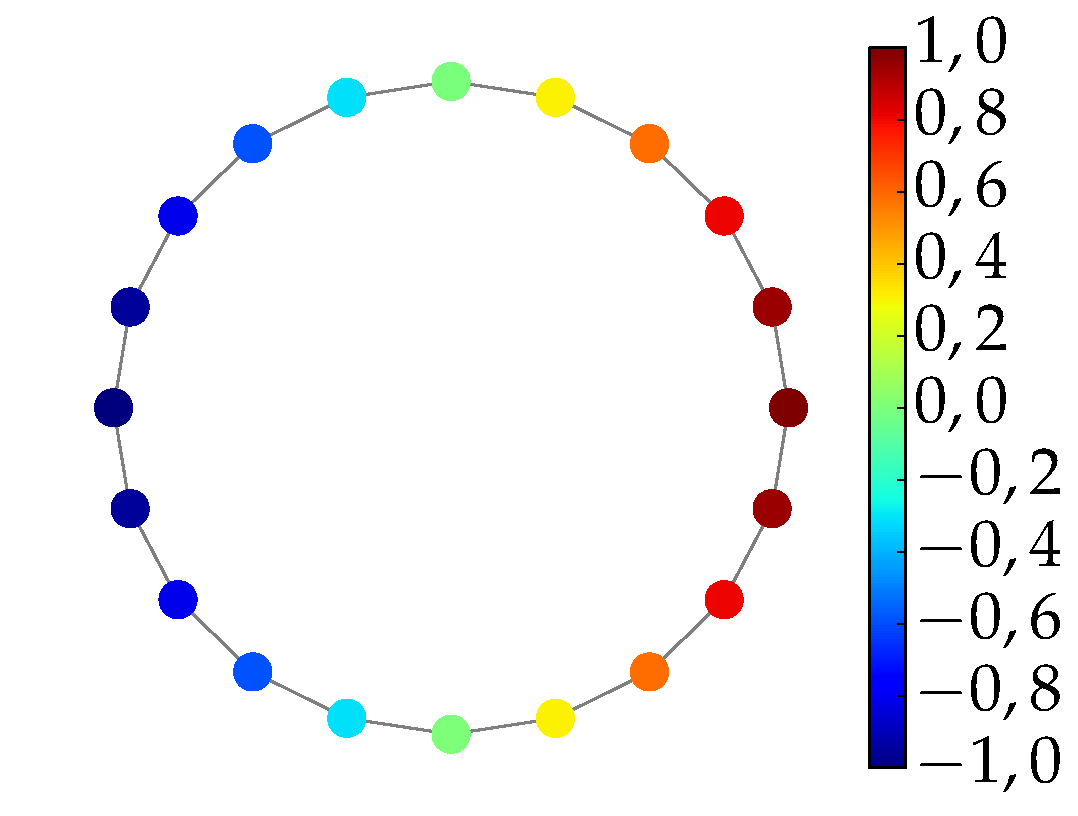
\includegraphics[width=\linewidth]{Figures/ring_different_structure_01_GSPA.pdf}
		}
	\end{minipage}~
	\begin{minipage}[c]{0.25\linewidth}
		\subfloat[\label{fig:diff_struct_b_GSPA}]{
			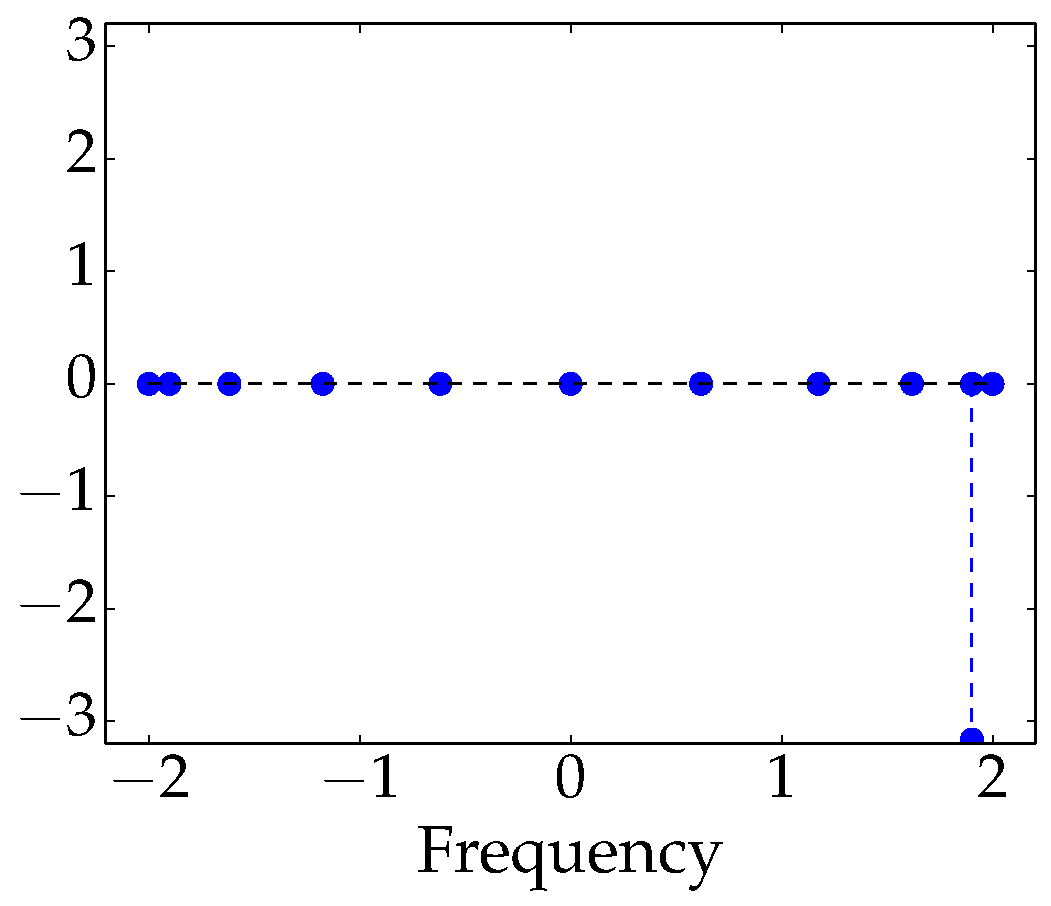
\includegraphics[width=\linewidth]{Figures/ring_different_structure_01_spectrum_GSPA_EN_2.pdf}
		}
	\end{minipage}%
	\floatsource
	\label{fig:diff_struct_GSPA}%
	\vspace{-0.2cm}
\end{figure}

The reader may have noticed a curious consequence from what was previously stated: unless the minimal and characteristic polynomials of $ \mathbf{A} $ are equal, the same frequency may be associated with two or more linearly independent frequency components, as indeed was the case in the example of Fig. \ref{fig:diff_struct_GSPA}. Furthermore, this figure shows that although the signal seems to be smooth, its frequency components are mostly associated with eigenvalues of high magnitude, what is counter-intuitive and provides a motivation to define a clear criterion to distinguish high and low graph frequencies.

The following mathematical reasoning consists of taking a metric which quantifies the expected signal smoothness, and use it to propose or confirm a notion of graph frequency. The metric used by Sandryhaila and Moura was the \emph{total variation}, taken from classical real analysis and defined for differentiable functions as \cite{rudin1987real,mallat1999wavelet}
\begin{equation}
%\label{key}
\Vert f \Vert_V = \int_{-\infty}^{\infty} |f'(t)| \mathrm{d}t.
\end{equation}

For discrete domain functions $ f_N[n] $, the Riemman integral is replaced by first order differences,
\begin{equation}
%\label{key}
\Vert f_N \Vert_V = \sum_p |f_N[n_p + 1] - f_N[n_p]|,
\end{equation}
which clearly quantifies the dissimilarity between contiguous values of the function $ f_N $. With this in mind, it was natural for Sandryhaila and Moura to use this metric in their attempt to quantify smoothness in GSP. Taking again the ring graph as a starting point, they looked at the total variation of a \textit{finite-length} discrete-time signal $ \mathbf{x} $:
\begin{equation}
\label{eq:TV}
TV(\mathbf{x}) = \sum_n | x_n - x_{(n-1) \text{ mod } N}|.
\end{equation}

From (\ref{eq:unit_shift}), one can see that (\ref{eq:TV}) may be written in terms of the $ \ell_1 $-norm\footnote{Throughout this text, the concepts of $ \ell_1 $- and $ \ell_2 $-norm will be frequently used. They are particular cases of the $ \ell_n $-norm of a vector $ \mathbf{x} \in \mathbb{C}^{N} $, defined as $ \Vert \mathbf{x}\Vert_n \overset{\Delta}{=} \left(\sum_{k=0}^{N-1} |x_k|^n\right)^{1/n} $.}
as $ TV(\mathbf{x}) = \Vert \mathbf{x} - \mathbf{C x}\Vert_1 $, by using the directed ring graph adjacency matrix to perform the cyclic shift. From that point, the generalization consisted of using this expression and defining the \emph{total variation on graphs} of a signal $ \mathbf{s} $ defined over the graph $ \mathcal{G} = \{\mathcal{V}, \mathbf{A}\} $ as
\begin{equation}
\label{eq:tv_graphs}
TV_G(\mathbf{s}) \overset{\Delta}{=} \Vert \mathbf{s} - \mathbf{A}^{\text{norm}} \mathbf{s}\Vert_1,
\end{equation}
with $ \mathbf{A}^{\text{norm}} = |\lambda_{max}|^{-1}\mathbf{A} $ and $ \lambda_{max} $ being the eigenvalue of $ \mathbf{A} $ having the highest absolute value. The normalization of the adjacency matrix aims to avoid the excessive magnification of the shifted signal \cite{sandryhaila2014frequency}.

\begin{figure}
	\centering
    \caption{Frequency ordering of graph signals, from low to high frequencies, in the complex plane.}
	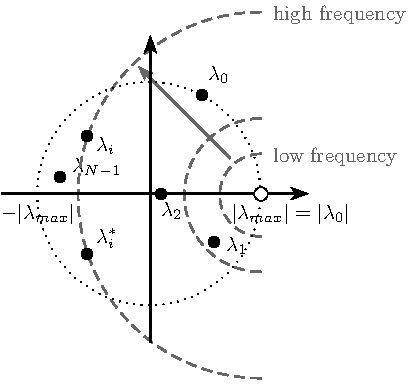
\includegraphics[width=0.45\linewidth]{Figures/graph_frequency_EN.pdf}
	\floatsource[adapted from \cite{sandryhaila2014frequency}]
	\label{fig:ordem_freq}
\end{figure}

Let $ \mathbf{A} $ be diagonalizable as in (\ref{eq:gft_01}) with (possibly complex) eigenvalues ordered like so
\begin{equation}
\label{eq:eig_order}
|\lambda_0| \leq |\lambda_1| \leq \dots \leq |\lambda_{N-1}| \overset{\Delta}{=} |\lambda_{max}|,
\end{equation}
associated with the eigenvectors $ (\mathbf{v}_i)_{i=0,\dots,N-1} $, scaled so that $ \Vert \mathbf{v}_i \Vert_1 = 1  \ \forall i$. Taking the total variation (on graphs) of the eigenvector $ \mathbf{v}_k $, one has
\begin{align*}
%\label{key}
TV_G(\mathbf{v}_k) &= \Vert \mathbf{v}_k - \mathbf{A} \mathbf{v}_k \Vert_1  = \Vert\mathbf{v}_k - \frac{1}{|\lambda_{max}|} \lambda_k \mathbf{v}_k \Vert_1 \notag \\
&= \left|1 - \frac{\lambda_k}{|\lambda_{max}|}\right| \Vert \mathbf{v}_k \Vert_1 = \Big| \lambda_k - |\lambda_{max}| \Big| \frac{\Vert \mathbf{v}_k \Vert_{1}}{|\lambda_{max}|}
\end{align*}
so that, since $ \Vert \mathbf{v}_k \Vert_1 = 1 $,
\begin{equation}
\label{eq:TV_ordering}
\Big| \! \lambda_i  - \! |\lambda_{max}|\Big| \! \leq \! \Big|  \lambda_j  - \! |\lambda_{max}|\Big| \! \! \iff \! \! TV_G(\mathbf{v}_i) \leq TV_G(\mathbf{v}_j),
\end{equation}
i.~e., frequency components associated with eigenvalues closer to the real point $ |\lambda_{max}| $ in the complex plane are \emph{smoother} (because they have lower total variation), and therefore are said to be of \emph{low frequency}. Fig. \ref{fig:ordem_freq} illustrates this ordering for graph frequencies, what clarifies the spectrum of the signal in Fig. \ref{fig:diff_struct_a_GSPA} (notice that since the graph is undirected, its adjacency matrix is symmetric and the eigenvalues are real-valued).


\begin{figure*}
	\centering
    \caption{(a) Directed sensor graph, with $ N=100 $ vertices and no loops or multiple edges. (b) Number of zero crossings and (b) total variation of the eigenvectors $ (\mathbf{v}_i)_{i=0,\dots,N-1} $ of the adjacency matrix $ \mathbf{A} $ of the graph in \emph{(a)}, ordered so that the respective eigenvalues appear from the closest to the farthest from the real point $ |\lambda_{max}| $ in the complex plane. That is, according to (\ref{eq:TV_ordering}) and Fig. \ref{fig:ordem_freq}, the eigenvectors are disposed in ascending order of frequency.}
	\subfloat[\label{fig:directed_graph}]{
			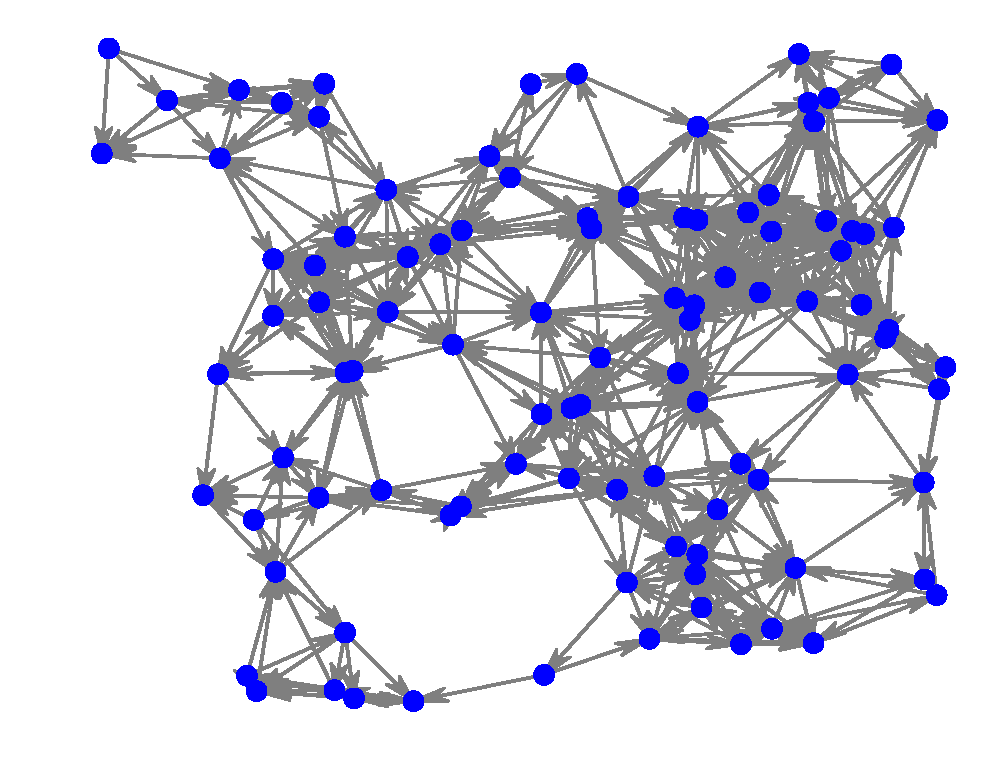
\includegraphics[width=0.31\linewidth]{Figures/showing_random_sensor_spectrum_directed_graph.pdf}
		}
	\subfloat[\label{fig:showing_random_sensor_spectrum_directed_b}]{
		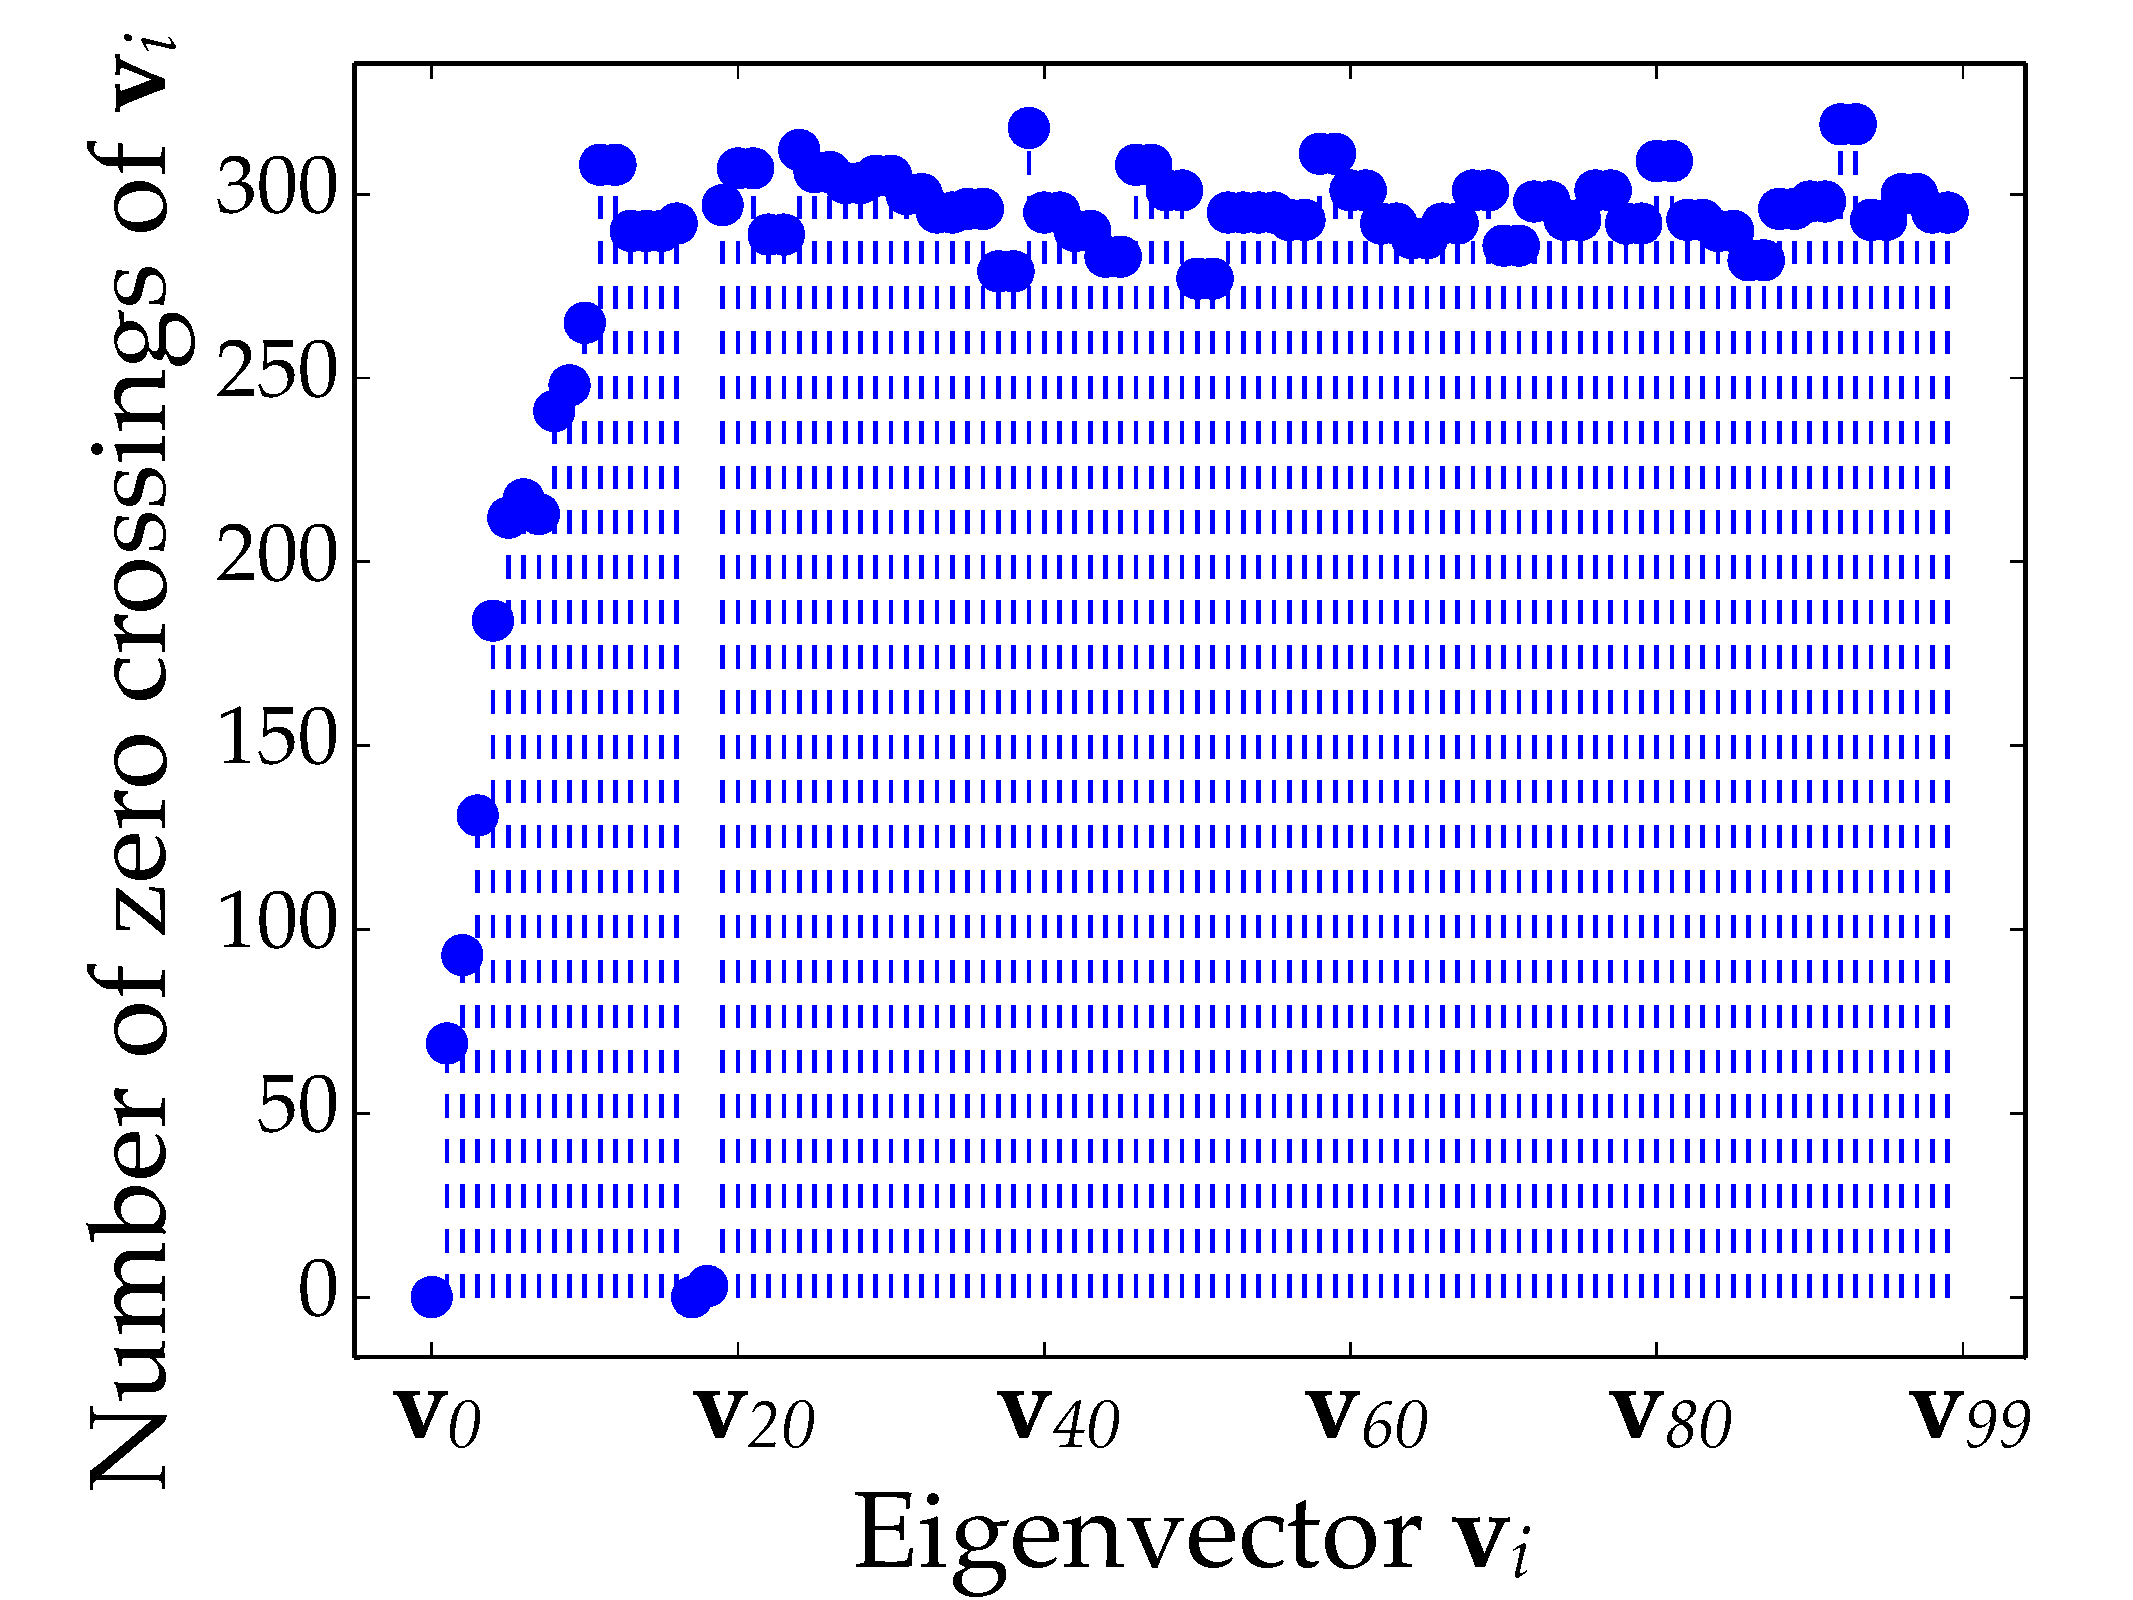
\includegraphics[width=0.33\linewidth]{Figures/showing_random_sensor_spectrum_directed_zero_crossings_1D_edited_EN.pdf}
	}~
	\subfloat[\label{fig:showing_random_sensor_spectrum_directed_c}]{
		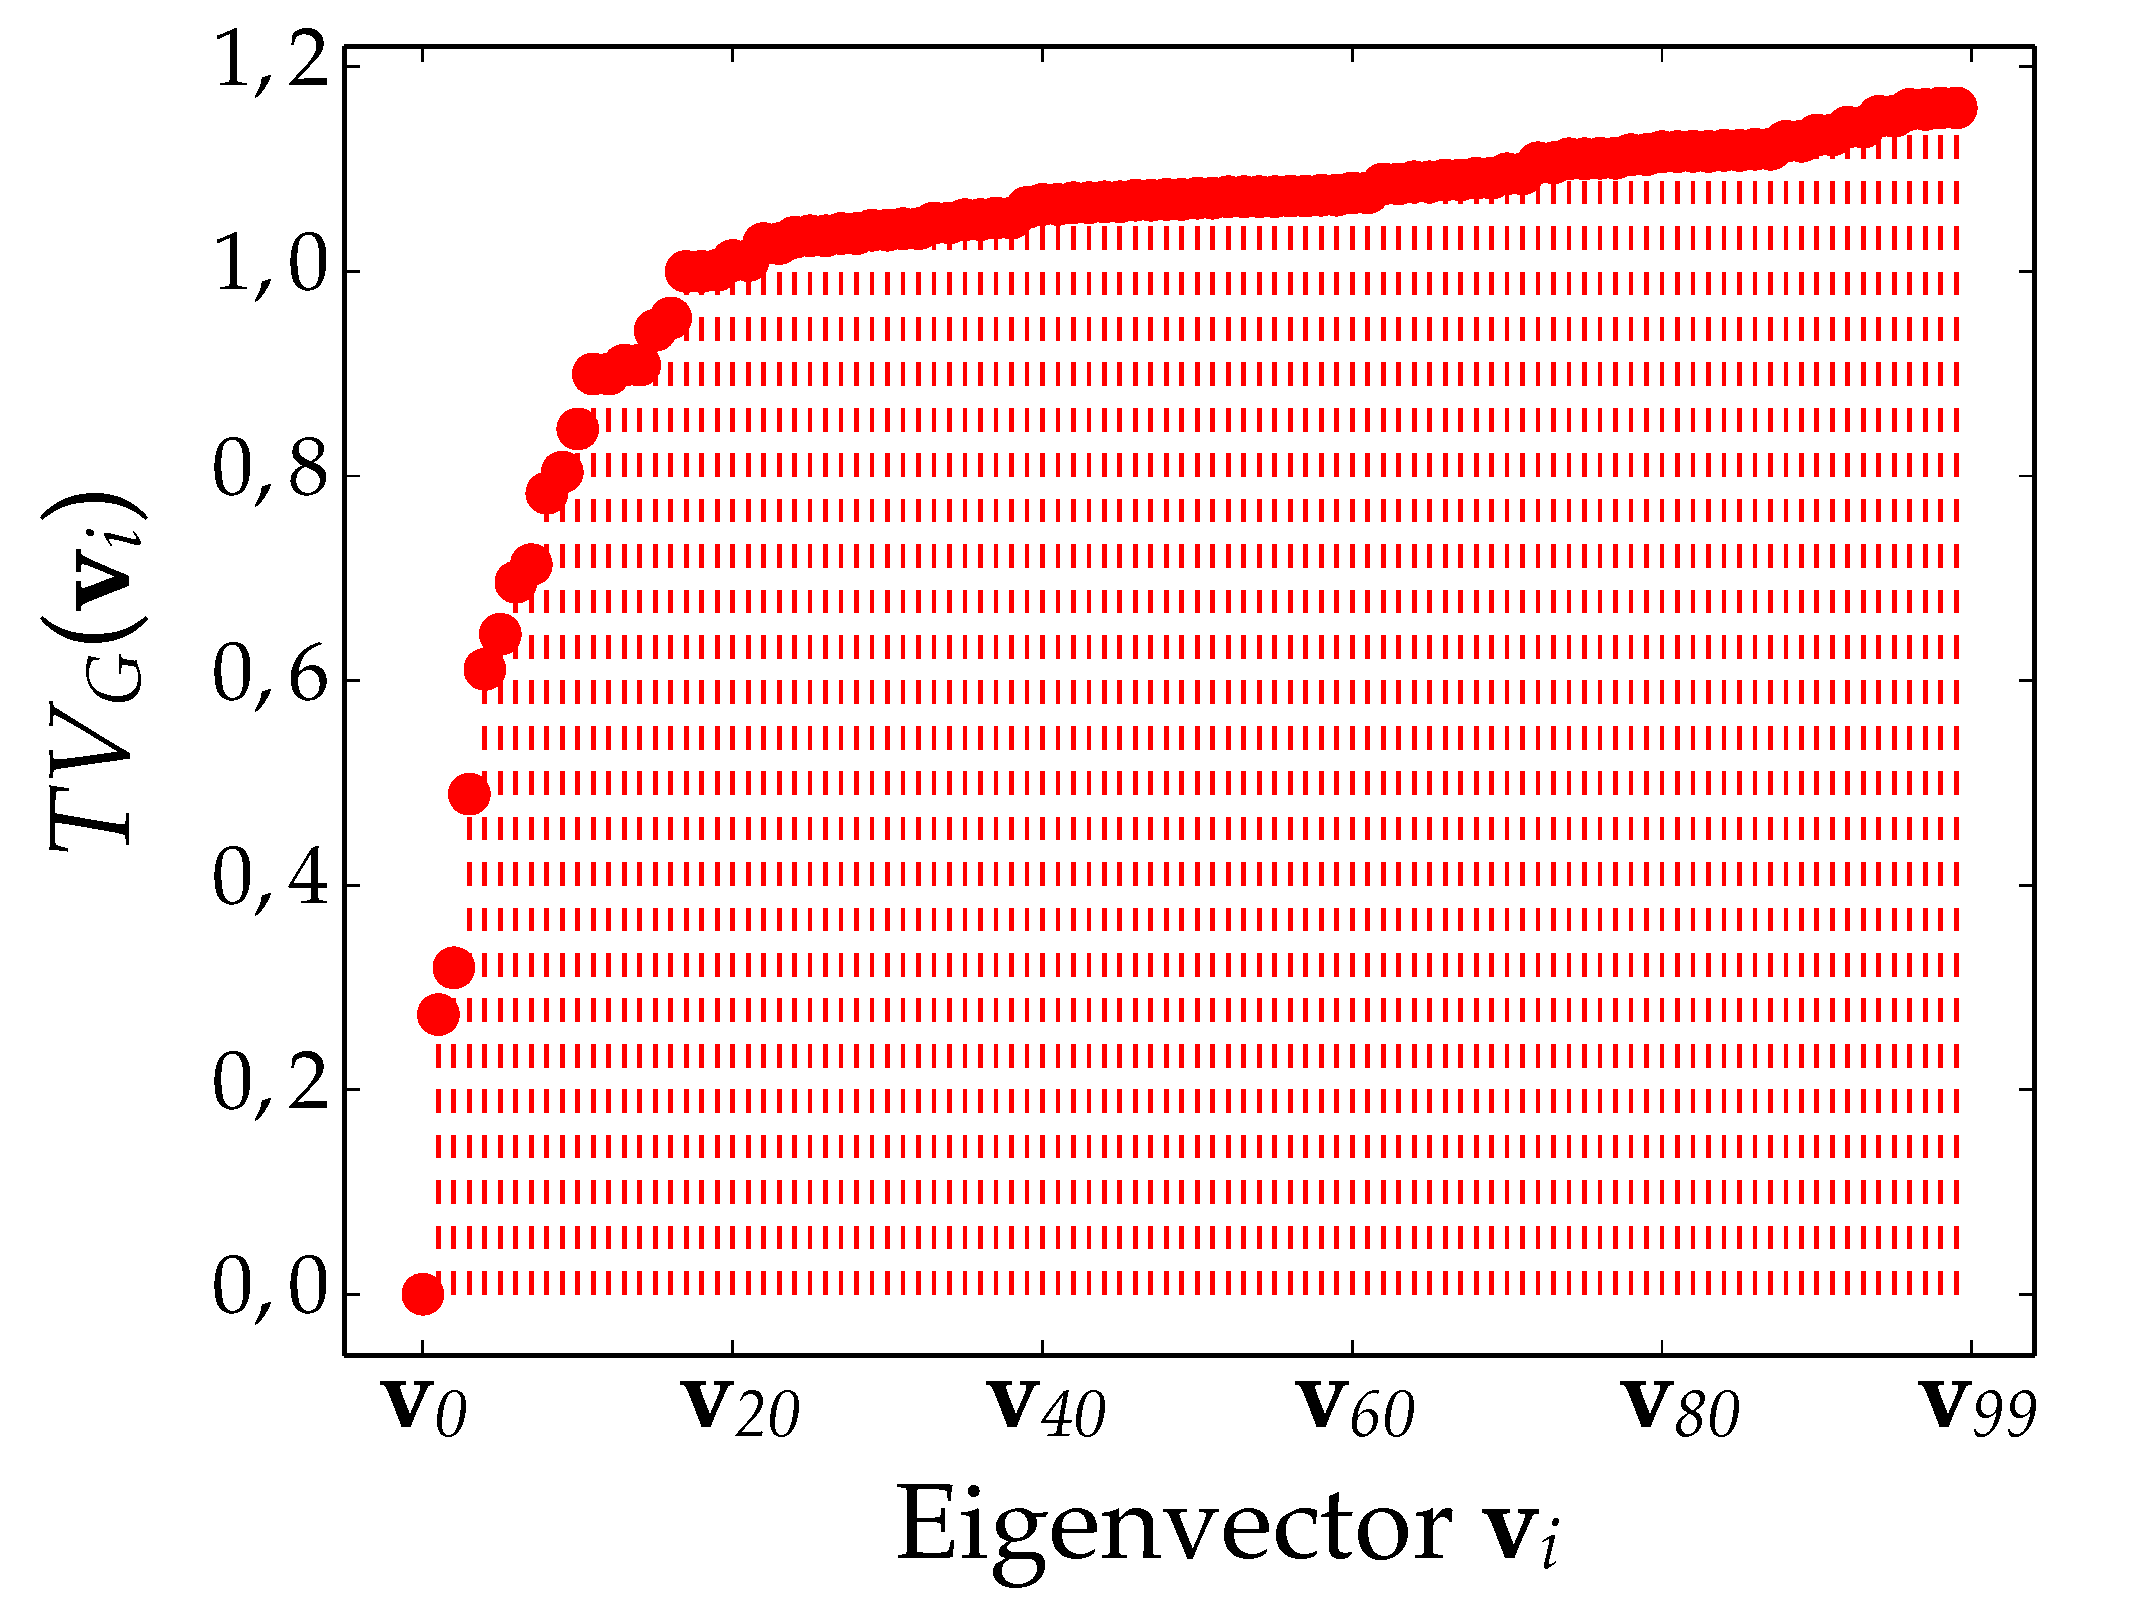
\includegraphics[width=0.33\linewidth]{Figures/showing_random_sensor_spectrum_directed_TV_1D_edited_EN.pdf}
	}
	\floatsource
	\label{fig:showing_random_sensor_spectrum_directed}
\end{figure*}

Let us take the directed graph in Fig. \ref{fig:directed_graph} to try to verify the consistency of the notion of frequency just derived. For this, along with the total variation on graphs, also the number of zero crossings (i.~e., the number of edges connecting vertices with signal samples of different sign) will be used to \emph{quantify} frequency. This quantity is also related to frequency in classical theory: the more a discrete signal has contiguous samples with different sign, generally the higher are its frequency components. These two functions, the total variation on graphs and the number of zero crossings, were calculated for each of the adjacency matrix eigenvectors, and the result is shown in Fig. \ref{fig:showing_random_sensor_spectrum_directed}, in which the eigenvectors $ \mathbf{v}_k $ are ordered in such a way that the respective eigenvalues $ \lambda_k $ appear from the closest to the farthest from the real point $ |\lambda_{max}| $ in the complex plane. Both metrics have similar behaviour, but since the number of zero crossings is indifferent to graph signal variations which do not change sign, it was already expected to be less accurate as a figure of merit for frequency. It matters to highlight, however, how the adopted eigenvector ordering indeed implies an ascending frequency order, since both functions in Fig. \ref{fig:showing_random_sensor_spectrum_directed_b} and \ref{fig:showing_random_sensor_spectrum_directed_c} agree on the tendency of growth. More than that, $ TV_G(\mathbf{v}_k) $ grows \emph{monotonically}, as it should do according to (\ref{eq:TV_ordering}).

It is convenient to conclude this discussion on the graph frequency domain by referring to the frequency response of graph filters. The definition given in Subsection \ref{subsec:filtros} considers the action of a matrix on a signal $ \mathbf{x} $ in the vertex domain of the graph $ \mathcal{G} = \{\mathcal{V}, \mathbf{A}\} $. In order to understand how the filter acts in the GFT domain, hereinafter called frequency domain, one may use (\ref{eq:gft_01}) and the polynomial representation of LSI filters. Let us take the filter $ \mathbf{H} =\sum_{\ell=0}^{L} h_\ell \mathbf{A}^\ell $ and its output to the input $ \mathbf{x} $ given by
\begin{align}\label{eq:resposta_freq_01}
\mathbf{H} \mathbf{x} &= \sum_{\ell=0}^{L} h_\ell \mathbf{A}^\ell \mathbf{x} =
\sum_{\ell=0}^{L} h_\ell \left(\mathbf{V} \mathbf{\Lambda} \mathbf{V}^{-1}\right)^\ell \mathbf{x} \notag \\
&= \mathbf{V} \left(\sum_{\ell=0}^{L} h_\ell \mathbf{\Lambda}^\ell \right) \mathbf{V}^{-1} \mathbf{x}.
\end{align}

Taking the GFT of both sides of the last equation yields
\begin{equation}\label{eq:resposta_freq_02}
\mathbf{V}^{-1} \mathbf{H} \mathbf{x} =
h(\mathbf{\Lambda}) \widehat{\mathbf{x}},
\end{equation}
which indicates that left-multiplication by $ \mathbf{H} $ (action of the filter in the vertex domain) is equivalent to the left-multiplication, in the frequency domain, by the matrix $ h(\mathbf{\Lambda}) $. In other words, $ h(\mathbf{\Lambda}) $ represents the frequency response of $ \mathbf{H} $.

\section{Summary}

This chapter guided the reader through the aspects regarding the fractional Fourier transform and graph signal processing most relevant to this work, closing the review of literature needed to have enough context to grasp and critique the chapters of original contributions that lie ahead. The key points to keep in mind are that
\begin{itemize}[noitemsep]
\item the fractional Fourier transform performs a real-valued rotation in the time-frequency plane,
\item the graph signal processing framework extends the usual discrete time domain to any network modeled by a graph, and as a consequence key basic concepts such as a unit shift must be redefined in terms of a graph matrix, called the graph shift operator,
\item the graph Fourier transform is the projection of a graph signal (vector) onto the space of eigenvectors of the graph shift operator.
\end{itemize}